\documentclass[12pt,fleqn]{article}

\usepackage{amsmath, amsthm, amssymb} %math expressions, theoreme/lemma, math symbols
\usepackage{mathtext} %russian letters in formulas

% fonts and lang
\usepackage{cmap}
\usepackage[T1, T2A]{fontenc}
\usepackage[utf8]{inputenc}
\usepackage[english, russian]{babel}

% formatting
\usepackage{geometry} %customize page layout
\geometry{left = 3cm}
\geometry{right = 1.5cm}
\geometry{top = 2cm}
\geometry{bottom = 2cm}

\usepackage{rotating}
\usepackage{minted}
\usepackage{mdframed}


\begin{document}
    \begin{titlepage}
        \begin{center}
            \textsf{\Large\bfseriesДокументация к библиотеке QComputations}\\[15mm]
        \end{center}
    \end{titlepage}

    \newpage

    \setcounter{page}{2}
	\thispagestyle{empty}
	\tableofcontents

    \newpage

    \section{Структура библиотеки}
        Идея данной библиотеки заключается в том, чтобы полностью избавить программиста от рутины реализации, оптимизации и параллелизации 
        при моделировании квантовых процессов. Сложность заключается в том, что каждый эксперимент и модель, по своей сути, уникальны. 
        Разные структуры состояний систем, способы их создания и генерации, разные операторы, разные численные методы моделирования и способы паралеллизации. Данная библиотека унифицирует всё это, 
        насколько это возможно к определённым базовым понятиям, с которыми потом и работает.

        Для начала нужно разобраться со вспомогательными классами, на которых основывается вся библиотека. Многоядерная версия (CPU\_CLUSTER) включает в 
        себя всё, что входит и в одноядерную (SINGLE), то есть, является расширением последней, поэтому сначала начнём с того, что входит в них обоих.

        \begin{itemize}

        \item{Основой всей библиотеки является класс \textbf{Matrix<T>}, который поддерживает типы \textbf{double} и \textbf{std::complex<double>}.
        Работа с ним упрощена настолько, насколько возможно. В нём реализованы все базовые операции и алгоритмы, часто используемые в 
        различного рода вычислениях. Подробное описание данного класса описано в главе \textbf{Прототипы функций и классов}. Реализация написана в файлах (все исходные файлы лежат в директории 
        \textsf{src/QComputations/}) \textsf{matrix.*}}

        \item{То, что я назвал ``дополнительными операторами''. Всякие удобные операторы, например умножение
        \textbf{std::vector<T>} на число типа \textbf{T}, умножение комплексной и вещественных матриц и так далее. Дополнительные операторы написаны в файлах \textsf{additional\_operators.*}}

        \item{Дополнительные функции. Например, является ли число нулём или \textbf{linspace} (точная копия из языка Python, и часто 
        используемый в программах).}

        \item{\textbf{QConfig} - конфигурационный синглтон (класс, который хранится в памяти в единственном экземпляре. Очень важная деталь библиотеки. Подробно описан в главе \textbf{QConfig}.)}

        \end{itemize}

        Далее идут ``основы'' , который есть только в MPI версии.

        Блочная матрица - класс \textbf{BLOCKED\_Matrix<T>}, также реализованы типы \textbf{double} и \textbf{std::complex<double>}.
        Данный класс предназначен для упрощённой работы с пакетом \textsf{Intel OneAPI} (без него MPI версия не работает). Реализация в файлах \textsf{blocked\_matrix.*}. Все прототипы функций, 
        кроме конструкторов, аналогичны одноядерной версии. Сам принцип работы можно посмотреть в документации к \textsf{Intel ScaLapack}.
        Данный класс упрощает всю работу с библиотекой, благодаря ему, вообще не нужно думать о программе на уровне ядер. Вся параллелизация 
        уже реализована в самом классе.

        Дополнительные MPI функции, по своей сути, упрощает работу с часто используемыми функциями в \textsf{Intel ScaLapack}. Используются в реализации 
        блочных матриц, и данный пакет довольно сложен в освоении, потому вообще не рекомендуется его трогать, но сами реализации вспомогательных к нему функций лежат
        в файлах \textsf{mpi\_functions.*}.

        Вообще, целью данной библиотеки является упрощение для программиста в принципе заниматься моделированием и вычислениями в данной сфере, 
        поэтому ``дополнительные операторы'', или, например, функции для MPI, скрываются ``под капотом''. Подразумевается, что Вы как раз и не должны
        думать о мудрёных \textsf{Intel MKL} и \textsf{Intel ScaLapack}, поэтому, вообще, неплохо бы знать только классы матриц и вспомогательных функций (Не MPI),
        остальные - для продвинутого пользования.

        Теперь разберём понятие, используемые в качестве абстракций для самих квантовых вычислений.

        Всё начинается с понятия состояния, по своей сути, оно определяет всю систему.
        Базовым понятием состояния является класс \textbf{Basis\_State}.
        Любой класс, являющийся наследником \textbf{Basis\_State}, принимается библиотекой. Реализация в файлах \textsf{state.*}
        Далее, я буду использовать класс \textbf{StateType}, для обозначения подобного класса.

        Сам класс \textbf{Basis\_State} включает в себя 2 главных понятия:
        \begin{enumerate}
            \item{Кудита - многозначного кубита, максимальное значение которого 
        также хранится в классе в массиве \textbf{max\_vals}.}
            \item{Группа кудитов: во многих системах очень удобно разделение кудитов на группы, как с точки зрения индексации, так и 
            с точки зрения математических нотаций. (В случае, когда оператор применяется к какой-то подсистеме, к остальным кудитам 
            применяется единичный оператор)}
        \end{enumerate}

        Начальное же состояние, которое может быть суперпозицией нескольких состояний, создаётся с помощью шаблонного класса 
        \textbf{State<StateType>}, то есть \textbf{StateType} - это какой-то элемент базиса, само 
        же общепринятое понятие состояния задаётся через \newline \textbf{State<StateType>}. 
        Примеры можно посмотреть в директории библиотеки \textsf{examples}, подробно о них написано в инструкции. На основе данного состояния будет дальше 
        генерироваться сам базис (данный процесс называется \textsf{Отбор рабочей области} (реализация в файлах \textsf{graph.*})).
        
        \textbf{Внимание! В State<StateType> нет автоматической нормализации данного вектора. Проверки на дураков также нет.}

        Следующее понятие, являющейся основой данной библиотеки: \textbf{Operator<StateType>}. Реализация в \textsf{quantum\_operators.*}. Данный класс предназначен для создания 
        собственных операторов и для их унификации. Работает это следующим образом.
        Вы пишите операторы в функциях следующего прототипа:
        \begin{center}

        \begin{mdframed}[linecolor=black, topline=true, bottomline=true,
            leftline=false, rightline=true]
            \begin{minted}[mathescape]{c++}
                State<Some_State> some_op(const Some_State& state);
            \end{minted}
        \end{mdframed}
        \end{center}

        После этого, вы создаёте сам ваш оператор следующим образом:

        \begin{mdframed}[linecolor=black, topline=true, bottomline=true,
            leftline=false, rightline=true]
            \begin{minted}[mathescape]{c++}
using OpType = Operator<Some_State>;
OpType H = OpType(some_op_1_1) * OpType(some_op_1_2) * ... * 
           OpType(some_op_1_n) * a_1 + 
           OpType(some_op_2_1) * OpType(some_op_2_2) * ... *
           OpType(some_op_2_n) * a_2 +
           ...
           OpType(some_op_m_1) * OpType(some_op_m_2) * ... *
           OpType(some_op_m_n) * a_m;
            \end{minted}
        \end{mdframed}

        \textsf{a\_i} - это комплексные числа (\textbf{std::complex<double>}).

        Данный оператор передаётся в конструктор гамильтониана. Можно также использовать напрямую для прогонки конкретного состояния
         через метод \textbf{run}, или неявно просто умножить на \textbf{State<StateType>}, или передать через оператор \textbf{()}.

        Далее идёт само понятие гамильтониана. Класс-конструкторы для гамильтониана от произвольного состояния: 
        \textbf{H\_by\_Operator<StateType>} для одноядерной версии и \newline
        \textbf{BLOCKED\_H\_by\_Operator<StateType>} для многоядерной. 
        В нём же генерируется базис.
        Также класс для задания через скалярное произведение \newline \textbf{H\_by\_Scalar\_Product<StateType>} и \newline \textbf{BLOCKED\_H\_by\_Scalar\_Product<StateType>}.
        В библиотеке также есть и готовые гамильтонианы и понятия состояний, например \textbf{TCH\_State} и \textbf{H\_TCH}, которые описаны
        в главе \textbf{Описание готовых состояний, гамильтонианов и операторов}.
        Все классы гамильтонианов являются наследниками класса \textbf{Hamiltonian} (для многоядерной версии \textbf{BLOCKED\_Hamiltonian}).
        Классы родители всегда работают только с состоянием \textbf{Basis\_State}, то есть, если вы вытащите базис из гамильтониана 
        методом \textbf{get\_basis}, вы получите \textbf{BasisType<Basis\_State>} (Реализация данного шаблонного класса для базиса лежит в 
        файле \textsf{state.hpp}. Вкраце, по своей сути, - это мудрёный \textbf{std::set<Basis\_State>}). Так сделано по причине экономии памяти и в принципе по другому унифицировать эффективно
        чисто программно невозможно. (На данном языке уж точно)
        
        Дальнейшее моделирование инвариантно относительно всех предыдущих понятий с точки зрения реализации и классов. Поэтому, моделирование  
        происходит с помощью отдельных функций и методов, работающие лишь с \textbf{State<Basis\_State>}, а также с \textbf{Hamiltonian}.
        Кастинг \textbf{StateType} к \textbf{Basis\_State}
        происходит автоматически. Примеры смотреть в \textsf{examples}.

        На данный момент реализованы методы (Подробнее в главе \textbf{Методы моделирования}):
            \begin{itemize}
                \item{Моделирование уравнения Шрёдингера через спектральное разложение. (\textbf{schrodinger})}
                \item{Моделирование основного квантового уравнения с помощью метода \textsf{Рунге-Кутта} 2 и 4 порядков.
                     (\textbf{quantum\_master\_equation}, выбор порядка метода происходит с помощью \textbf{QConfig}. (по умолчанию 2))}
            \end{itemize}
        Результаты этих методов в дальнейшем визуализируется либо напрямую в самой библиотеке в версиях с \textsf{Python API}, либо через файловую систему и дополнительный скрипт, путь к 
        которому будет храниться после установки в переменной окружения \textsf{\$SEABORN\_PLOT}. (Настройки к нему в переменной 
        \textsf{\$SEABORN\_CONFIG})
        Об этом подробно написано в главе \textbf{Визуализация}.

        Для более детального понимания, приведена схема зависимостей внутри стуктуры данной библиотеки.

        \begin{figure}[H]
			\makebox[\textwidth]{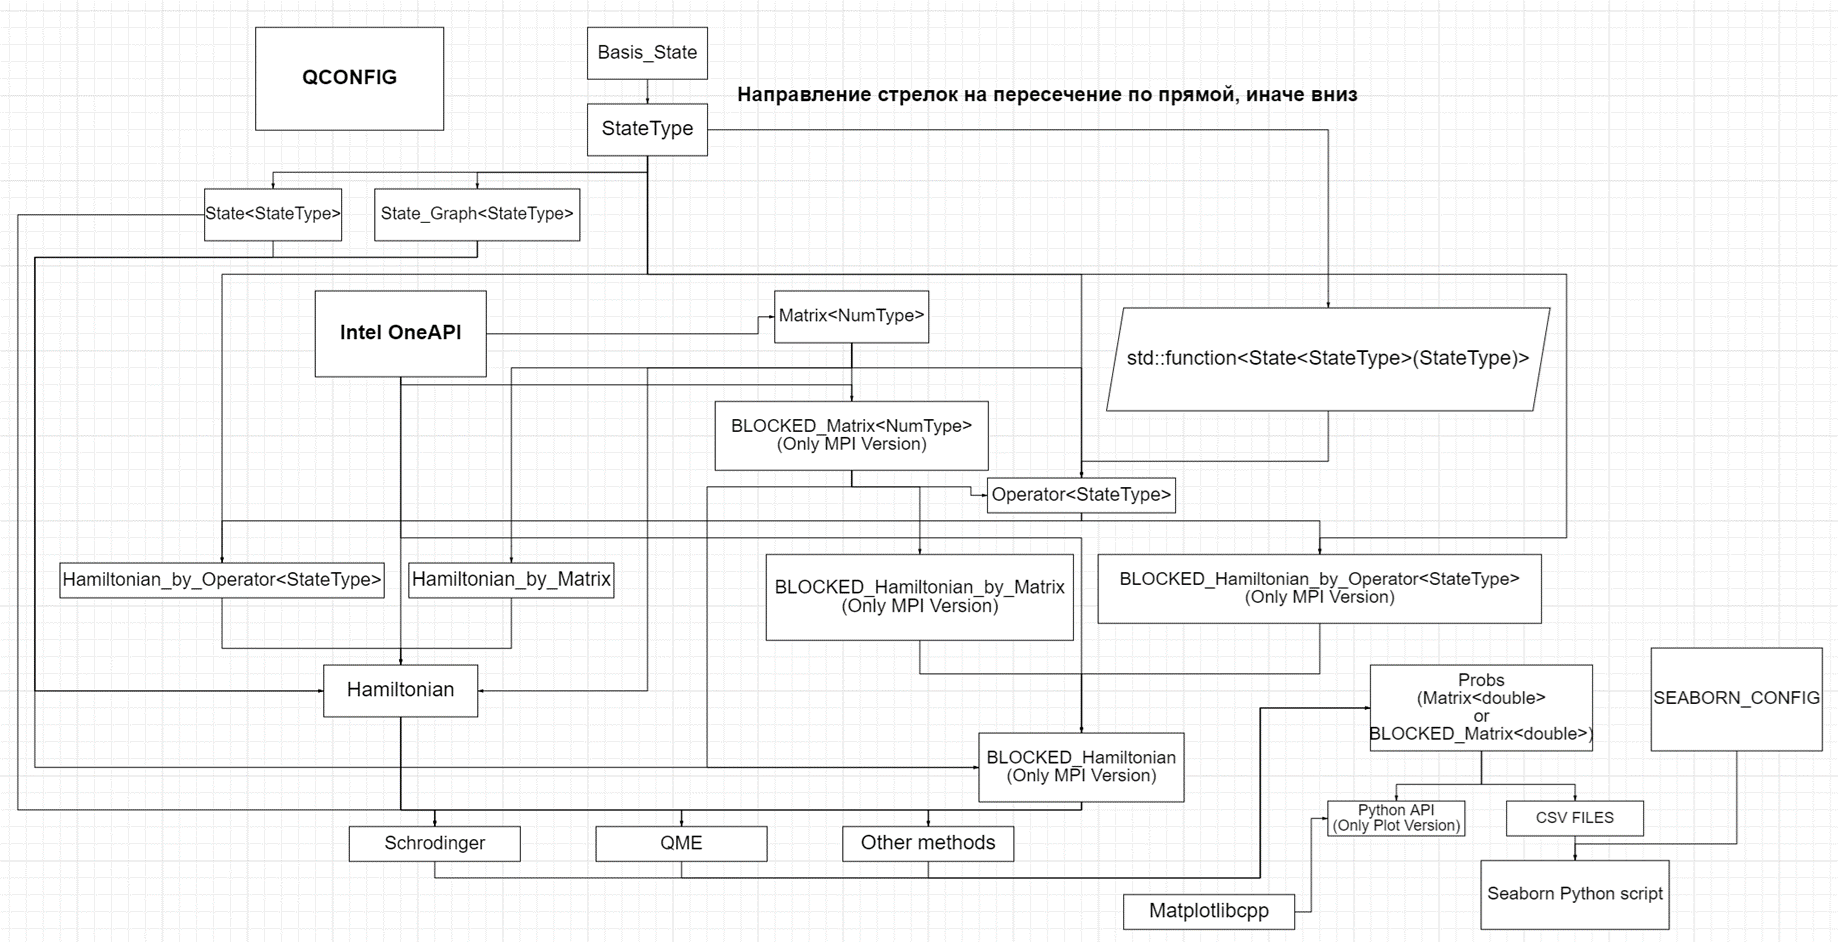
\includegraphics[width=0.9\paperwidth, height=0.4\textheight]{./images/structure.png}}
			\caption{\label{structure} Взаимосвязи классов в библиотеке \textbf{QComputations} между собой.}
        \end{figure}

        Библиотека, на данный момент, делится на 4 версии:
        \begin{enumerate}
            \item{Версия на одном ядре с поддержкой графиков \newline (\textsf{libQComputations\_SINGLE.so})}
            \item{Версия на одном ядре без поддержки графиков \newline (\textsf{libQComputations\_SINGLE\_NO\_PLOTS.so})}
            \item{Версия на многих ядрах с поддержкой графиков\newline (\textsf{libQComputations\_CPU\_CLUSTER.so})}
            \item{Версия на многих ядрах без поддержки графиков \newline
            (\textsf{libQComputations\_CPU\_CLUSTER\_NO\_PLOTS.so})}
        \end{enumerate}

        2 и 4 версии предполагают использование файловой системы для хранения результатов, они сохраняют в указанные программистом директории 
        файлы в формате CSV. Визуализация этих данных происходит с помощью скрипта \textbf{seaborn\_plot.py} на языке Python, путь к которому, 
        после установки библиотеки, будет хранится в переменной окружения \textsf{\$SEABORN\_PLOT}. Инструкция использования данного скрипта
        находится в главе \textbf{Визуализация}.

        Библиотека делится на 2 типа (на данный момент): последовательная/одноядерная (1, 2) и MPI (3, 4). В MPI также полностью входит одноядерная версия, поэтому можно комбинировать 
        методы параллелизации между собой, например параллелить набор не блочных гамильтонианов по ним же самим.

    \section{\textbf{QConfig}}
    \textbf{QConfig} - это синглтон (класс, хранящийся в памяти в единственном экземпляре). Одна из главных проблем квантовых вычислений - очень большое количество констант и переменных,
    которые можно регулировать. Все они взаимосвязаны, и если не уследить за этим, то можно получить некорректный результат, который очень часто будет выглядеть правдоподобным.
    Изначально \textbf{QConfig} предназначался для них, впоследствии оказалось, что данная идея куда более удобная. С его помощью можно настраивать не только константы, но и 
    всю библиотеку целиком, при этом не нужно будет ничего перекомпилировать или переустанавливать.
    Статичная библиотека, в том плане, что есть неизменные функции, классы, методы и так далее мало на что претендует в области квантовой механики.
    \textbf{QConfig} делает \textbf{QComputations} более динамичной в этом отношении. С его помощью можно выбирать алгоритмы моделирования, не меняя в принципе абстрактно сам метод моделирования.
    (Например, хотим моделировать эволюции основным квантовым уравнением (функция \textbf{quantum\_master\_equation}), но хотим моделировать его
    \textsf{Рунге-Куттом} 4 порядка, а не 2, тогда здесь и появляется \textbf{QConfig})

    Если резюмировать, \textbf{QConfig} - это класс-синглтон для настройки констант и всей библиотеки в целом.

\begin{mdframed}[linecolor=black, topline=true, bottomline=true,
    leftline=false, rightline=false]
\begin{minted}[mathescape]{c++}  
enum FUNCTION_QME {RUNGE_KUTT_4 = 121, RUNGE_KUTT_2 = 122};

// Значения по умолчанию
namespace {
    // Параметры figure из matplotlib Python
    // Только для версии со встроенным Python API
    enum FIG_PARAMS {FIG_WIDTH = 19, FIG_HEIGHT = 10, DPI = 80};

    // Значение постоянной планка
    constexpr double h_default = 1;
    // Значение частоты
    constexpr double w_default = 1;
    // Значение силы взаимодействия частиц с полем
    constexpr double g_default = 0.01;
    // Значение длины волновода (Для реализации TCH_State)
    constexpr double waveguides_length_default = 2*M_PI;
    // Значение амплитуды волновода (Для реализации TCH_State)
    constexpr double waveguides_amplitude_default = 0;
    // Максимальное число фотонов (Для реализации TCH_State)
    constexpr int max_photons_default = 1;

    // Значение epsilon
    constexpr double eps_default = 1e-12;
    // Значение ширины для вывода матриц в stdout
    constexpr int width_default = 15;

    // Число символов для одного числа при записи в файл
    constexpr int csv_max_number_size_default = 21;
    // Количество цифр после запятой
    constexpr int csv_num_accuracy_default = 16;

    // Алгоритм по умолчанию для моделирования КОУ
    constexpr FUNCTION_QME qme_algorithm_default = RUNGE_KUTT_2;
}

class QConfig {
    public:
        // Реализация синглтона
        QConfig(const QConfig&) = delete;
        void operator=(const QConfig&) = delete;

        static QConfig& instance() {
            static QConfig instance;
            return instance;
        }

        
        // Методы для установки значений 
        void set_h(double h) { h_ = h; }
        void set_max_photons(int max_photons) 
             { max_photons_ = max_photons; }
        void set_w(double w) { w_ = w; }
        void set_g(double g) { g_ = g; }
        void set_fig_width(int fig_width) 
              { fig_width_ = fig_width; }
        void set_fig_height(int fig_height)
              { fig_height_ = fig_height; }
        void set_dpi(int dpi)
              { dpi_ = dpi; }
        void set_eps(double eps)
              { eps_ = eps; }
        void set_width(int width)
              { width_ = width; }
        void set_waveguides_length(double waveguides_length)
              { wavegiudes_length_ = waveguides_length; }
        void set_csv_max_number_size(int csv_max_number_size)
              { csv_max_number_size_ = csv_max_number_size; }
        void set_csv_num_accuracy(int csv_num_accuracy)
              { csv_num_accuracy_ = csv_num_accuracy; }

        // Методы для получения значений
        double h() const { return h_; }
        int max_photons() const { return max_photons_; }
        double w() const { return w_; }
        double g() const { return g_; }
        int fig_width() const { return fig_width_; }
        int fig_height() const { return fig_height_; }
        int dpi() const { return dpi_; }
        double eps() const { return eps_; }
        int width() const { return width_; }
        int E_LEVELS_COUNT() const { return E_LEVELS_COUNT_; }
        double waveguides_length() const { return wavegiudes_length_; }
        double waveguides_amplitude() const { return wavegiudes_amplitude_; }
        int csv_max_number_size() const { return csv_max_number_size_; }
        int csv_num_accuracy() const { return csv_num_accuracy_; }
    private:
        QConfig() {}
        ~QConfig() {} // Память освобождается в конце программы
        int fig_width_ = int(FIG_WIDTH);
        int fig_height_ = int(FIG_HEIGHT);
        int dpi_ = int(DPI);
        
        int csv_max_number_size_ = csv_max_number_size_default;
        int csv_num_accuracy_ = csv_num_accuracy_default;

        int width_ = width_default;

        double eps_ = eps_default;
        
        int max_photons_ = max_photons_default;
        double wavegiudes_length_ = waveguides_length_default;
        double wavegiudes_amplitude_ = waveguides_amplitude_default;
    
        double h_ = h_default;
        double w_ = w_default;
        double g_ = g_default;
};
\end{minted}
\end{mdframed}
    \section{Прототипы функций и классов}

        Здесь рассматриваются только сами классы и их методы. Саму детальную реализацию смотреть в исходный файлах (\textsf{src/QComputations/}).

        В местах, где можно вставить тип \textbf{double} или \textbf{std::complex<double>}, будет написано \textbf{NumType} или \textbf{T}.

        \subsection{Обычная матрица \textbf{Matrix<T>}}
        \textbf{matrix\_style} - хранения матрицы по строкам (Си стиль - \textbf{C\_STYLE}) или по столбцам (Фортрановский стиль - \textbf{FORTRAN\_STYLE}).
        Файлы \textsf{matrix.*}.

            \begin{mdframed}[linecolor=black, topline=true, bottomline=true,
                leftline=false, rightline=false]
            \begin{minted}[mathescape]{c++}
enum MATRIX_STYLE { C_STYLE = 120, FORTRAN_STYLE = 121 };

template<typename T> class Matrix {
    public:
        Matrix() = default;
        // Иницианилизирует матрицу размера n x m 
        // (n - число строк, m - число столбцов)
        explicit Matrix(MATRIX_STYLE matrix_style, size_t n, size_t m);
        
        // Иницианилизирует матрицу размера n x m с начальным 
        // значением во всех элементах init_val
        explicit Matrix(MATRIX_STYLE matrix_style, size_t n, size_t m,
                        const T& init_val);

        // Конструктор копирования
        explicit Matrix(const Matrix<T>& A);

        // Если у вас хранится одномерный массив, его можно 
        // привести к виду матрицу, указав размер n и m.
        explicit Matrix(const std::vector<T>& mass, size_t n, size_t m, 
                        MATRIX_STYLE matrix_style);

        // Создать матрицу, с помощью функции типа
        // std::function<COMPLEX(size_t i, size_t j)>, 
        // где i и j координаты ячеек матрицы.
        explicit Matrix(MATRIX_STYLE matrix_style, size_t n, size_t m, 
                        std::function<COMPLEX(size_t, size_t)> func);

        // Привести матрицу к другому типу (реализацию оставил для понимания)
        template<typename V>
        Matrix(const Matrix<V>& A): n_(A.n()), m_(A.m()) {
            for (size_t i = 0; i < n_; i++) {
                for (size_t j = 0; j < m_; j++) {
                    mass_.emplace_back(static_cast<V>(A[i][j]));
                }
            }

            matrix_style_ = A.get_matrix_style();
        }

        // Привести матрицу вида вектора векторов к нашему
        explicit Matrix(const std::vector<std::vector<T>>& A, 
                        MATRIX_STYLE matrix_style);

        Matrix<T>& operator=(const Matrix<T>& A);

        // Вместо строки под номером index вставить строку v
        void modify_row(size_t index, const std::vector<T>& v);

        // Вместо столбца под номером index вставить строку v
        void modify_col(size_t index, const std::vector<T>& v);

        // Получить строку
        std::vector<T> row (size_t index) const;
        // Получить столбец
        std::vector<T> col (size_t index) const;

        size_t n() const { return n_; } // Число строк
        size_t size() const { return n_; } // удобно для квадратных матриц
        size_t m() const { return m_; } // Число столбцов

        // Увеличить число строк в матрице
        void add_rows(size_t row_count);

        // Увеличить число столбцов в матрице
        void add_cols(size_t col_count);

        // Удалить число строк в матрице
        void remove_rows(size_t row_count);

        // Удалить число столбцов в матрице
        void remove_cols(size_t col_count);

        void expand(size_t n); // add_rows + add_cols
        void reduce(size_t n); // remove_rows + remove_cols

        // Не добавлять шаблонные виды операторов для матриц
        Matrix<T> operator* (const Matrix<T>& A) const;
        Matrix<T> operator+ (const Matrix<T>& A) const;
        Matrix<T> operator- (const Matrix<T>& A) const;

        Matrix<T>& operator+=(const Matrix<T>& A);
        Matrix<T>& operator-=(const Matrix<T>& A);

        std::vector<T> operator* (const std::vector<T>& v) const;

        void operator*= (const T& num);

        Matrix<T> operator* (const T& num) const;
        Matrix<T> operator+ (const T& num) const;
        Matrix<T> operator- (const T& num) const;
        Matrix<T> operator/ (const T& num) const;
        void operator/= (const T& num);

        bool operator==(const Matrix<T>& A) const;

        // Вернуть матрицу в хранимом виде (в виде вектора)
        std::vector<T>& get_mass() { return mass_; }
        std::vector<T> get_mass() const { return mass_; }

        // Вернуть указатель на массив
        T* data() { return mass_.data(); }
        const T* data() const { return mass_.data(); }

        Matrix<T> transpose() const;
        Matrix<T> hermit() const;
        void show(size_t width = QConfig::instance().width()) const;
    
        // (!!!) Индексация для С стиля
        T* operator[](size_t index_row) { return mass_.data() + index_row * m_; }; 
        const T* operator[](size_t index_row) const { 
            return mass_.data() + index_row * m_; };
    
        // (!!!) Инддексация для Фортрановского стиля
        T& operator()(size_t index_row, size_t index_col) { 
            return mass_.data()[index_col * n_ + index_row]; }
        const T operator()(size_t index_row, size_t index_col) const { 
            return mass_.data()[index_col * n_ + index_row]; }
    
        // Лидирующее измерение
        size_t LD() const { return (matrix_style_ == C_STYLE ? m_ : n_); }

        bool is_c_style() const { return matrix_style_ == C_STYLE; }
        MATRIX_STYLE get_matrix_style() const { return matrix_style_; }

        // Привести матрицу к нужному стилу расположения в памяти
        // !! Нужно быть внимательным при индексации с помощью [] и () !!
        void to_fortran_style();
        void to_c_style();

        // Вернуть подматрицу размера n x m, начало которой 
        // находится по координатам row_index, col_index
        Matrix<T> submatrix(size_t n, size_t m, size_t row_index, 
                            size_t col_index) const;

        // Индексация общего вида, независимо от стиля матрицы
        size_t index(size_t i, size_t j) const { if (matrix_style_ == C_STYLE) 
                                                return i * m_ + j; 
                                                else 
                                                return j * n_ + i; }

        // Получить элемент матрицы, с помощью которого также можно менять матрицу
        T& elem(size_t i, size_t j) { 
            return mass_.data()[this->index(i, j)]; }
        const T elem(size_t i, size_t j) const { 
            return mass_.data()[this->index(i, j)]; }

        // Записать матрицу в файл, в формате CSV. Точность 
        // регулируется с помощью QConfig.
        void write_to_csv_file(const std::string& filename) const;
    private:
        size_t n_; // Число строк
        size_t m_; // Число столбцов
        std::vector<T> mass_; // Массив с данными
        MATRIX_STYLE matrix_style_; // Стиль матрицы - 
                                    // по умолчанию С стиль.
};
            \end{minted}
            \end{mdframed}
        \subsection{Блочная матрица \textbf{BLOCKED\_Matrix<T>}}

        Блочная матрица напрямую связана с решёткой \textsf{BLACS} (придумка \textsf{Intel OneAPI}). Тип \textbf{ILP\_TYPE} в библиотеке - это тип, зависящий от того, 
        с помощью какой версий библиотек \textsf{Intel OneAPI} идёт компиляция, подробнее смотреть в самой документации \textsf{Intel OneAPI}. На данный момент библиотека компилируется
        с обычными библиотеками, и \textbf{ILP\_TYPE=int}. Реализована вспомогательная функция для инициализации решётки \textsf{BLACS} - \textbf{init\_grid()}.

        \textbf{MATRIX\_TYPE} - это перечисляемый тип:

        \begin{mdframed}[linecolor=black, topline=true, bottomline=true,
            leftline=false, rightline=false]
        \begin{minted}[mathescape]{c++}
            enum MATRIX_TYPE { GE = 120, SY = 121, HE = 122};
        \end{minted}
        \end{mdframed}

        GE - обычная матрица. SY - симметричная. HE - эрмитовая. Как не покажется странным, в пакете Intel OneAPI нет экономии памяти на случай последних двух.
        Элементы нижней треугольной части просто не инициализируются. (Причём обязательно)

        Также блоки хранятся только и только в Фортрановском стиле (в памяти расположены по столбцам).

        \textbf{ПРЕДУПРЕЖДЕНИЕ. ПРИ НЕ КВАДРАТНЫХ РАЗМЕРАХ БЛОКОВ (NB, MB) НЕ РАБОТАЕТ ЭРМИТОВОЕ РАЗЛОЖЕНИЕ МАТРИЦЫ. ВЫДАЁТ НЕКОРРЕКТНУЮ ОШИБКУ.}


        \begin{mdframed}[linecolor=black, topline=true, bottomline=true,
            leftline=false, rightline=false]
        \begin{minted}[mathescape]{c++}
template <typename T>
class BLOCKED_Matrix {
    public:
        explicit BLOCKED_Matrix() = default;

        // Скопировать блочную матрицу А,
        // но с новым локальным блоком local_matrix.
        explicit BLOCKED_Matrix(const BLOCKED_Matrix<T>& A, 
                                const Matrix<T>& local_matrix);

        // Сгенерировать матрицу с помощью функции. NB и MB 
        // - размеры блоков (подблоков общего блока, 
        // так как блок в ядре генерируется циклически, 
        // подробнее в документации к Intel OneAPI), 
        // значения 0 означает выбор размера 
        // блока по умолчанию. (Рекомендуется)
        explicit BLOCKED_Matrix(ILP_TYPE ctxt, MATRIX_TYPE type, 
                                size_t n, size_t m, 
                                std::function<T(size_t, size_t)> func, 
                                size_t NB = 0, size_t MB = 0);

        // Сгенерировать матрицу с начальным значанием value
        explicit BLOCKED_Matrix(ILP_TYPE ctxt, MATRIX_TYPE type, 
                                size_t n, size_t m, T value, 
                                size_t NB = 0, size_t MB = 0);

        // Сгенерировать неинициализированную матрицу
        explicit BLOCKED_Matrix(ILP_TYPE ctxt, MATRIX_TYPE type, 
                                size_t n, size_t m, 
                                size_t NB = 0, size_t MB = 0);

        // Распределить матрицу А по блокам
        explicit BLOCKED_Matrix(ILP_TYPE ctxt, MATRIX_TYPE type, 
                                const Matrix<T>& A, 
                                size_t NB = 0,  size_t MB = 0);

        // Создать пустую матрицу по
        // размерностям результата перемножения матриц A и B
        explicit BLOCKED_Matrix(const BLOCKED_Matrix<T>& A, 
                                const BLOCKED_Matrix<T>& B);

        // Получить элемент по глобальным индексам i и j. 
        // (Требует участия как минимум 2 процессов. 
        // Того, который спрашивает, и того, у кого 
        // находится блок с данным элементом, участие 
        // остальных позволяется, но необязательно)
        T get(size_t i, size_t j) const;

        // Установить элемент по глобальным индексам i и j 
        // значению num. (Требует участия 
        // как минимум 2 процессов. Того, который приказывает 
        // установить элемент, и того, у кого находится 
        // блок с данным элементом)
        void set(size_t i, size_t j, T num);

        // Операторные функции. Главная цель - чтобы работать 
        // с данным классом было также легко, как с обычной матрицей.
        BLOCKED_Matrix<T> operator*(const BLOCKED_Matrix<T>& B) const;
        void operator*=(const BLOCKED_Matrix<T>& B);
        BLOCKED_Matrix<T> operator*(T num) const;
        void operator*=(T num);
        BLOCKED_Matrix<T> operator+(const BLOCKED_Matrix<T>& B) const;
        void operator+=(const BLOCKED_Matrix<T>& B);
        BLOCKED_Matrix<T> operator+(T num) const;
        void operator+=(T num);
        BLOCKED_Matrix<T> operator-(const BLOCKED_Matrix<T>& B) const;
        void operator-=(const BLOCKED_Matrix<T>& B);
        BLOCKED_Matrix<T> operator-(T num) const;
        void operator-=(T num);
        BLOCKED_Matrix<T> operator/(T num) const;
    
        // Вернуть локальный размер общего блока матрицы (число строк)
        size_t local_n() const { return local_matrix_.n(); }

        // Вернуть локальный размер общего блока матрицы (число столбцов)
        size_t local_m() const { return local_matrix_.m(); }

        // Вернуть глобальное число строк в матрице
        size_t n() const { return n_; }

        // Вернуть глобальное число столбцов в матрице
        size_t m() const { return m_; }

        // Вернуть число строк в подблоках
        size_t NB() const { return NB_; }

        // Вернуть число столбцов в подблоках
        size_t MB() const { return MB_; }

        // Вернуть BLACS сontext
        ILP_TYPE ctxt() const { return ctxt_; }

        // Вернуть тип матрицы
        MATRIX_TYPE matrix_type() const { return matrix_type_; }

        // Вернуть весь общий блок в виде одномерного массива
        Matrix<T>& get_local_matrix() { return local_matrix_;}
        const Matrix<T>& get_local_matrix() const { return local_matrix_;}

        // Вернуть указатель на локальный элемент по локальным индексам i и j.
        T* data(size_t i = 0, size_t j = 0) { 
            return local_matrix_.data() + get_local_index(i, j); }
        const T* data(size_t i = 0, size_t j = 0) const { 
            return local_matrix_.data() + get_local_index(i, j); }

        // Вернуть локальный элемент по локальный индексам i и j.
        T& operator()(size_t i, size_t j) { return local_matrix_(i, j); }
        const T operator()(size_t i, size_t j) const { return local_matrix_(i, j); }

        // Распечатать матрицу в блочной виде, 
        // то есть каждый процесс напечатает свой блок
        void print_distributed(const std::string& name) const;

        // Распечатать матрицу в виде обычной матрицы
        void show(size_t width = QConfig::instance().width(), 
                  ILP_TYPE root_id = mpi::ROOT_ID) const;

        // Записать матрицу в файл формата CSV
        void write_to_csv_file(const std::string& filename) const;

        // Получить глобальный номер измерения по локальному
        ILP_TYPE get_global_row(size_t i) const;
        ILP_TYPE get_global_col(size_t j) const;

        // Получить локальный номер измерения по глобальному
        ILP_TYPE get_local_row(size_t i) const;
        ILP_TYPE get_local_col(size_t j) const;

        // Получить строку в BLACS, в которой находится ядро, 
        // которому принадлежит строка под номером i.
        ILP_TYPE get_row_proc(size_t i) const;

        // Получить столбец в BLACS, в которой находится ядро, 
        // которому принадлежит столбец под номером j.
        ILP_TYPE get_col_proc(size_t j) const;

        // Сделать эрмитовое преобразование матрице
        BLOCKED_Matrix<T> hermit() const;

        // Получить весь столбец целиком
        std::vector<T> col(size_t i) const;

        // Получить всю строку целиком
        std::vector<T> row(size_t j) const;

        // Важный элемент библиотеки Intel OneAPI, но для 
        // пользователя библиотеки QComputations бесполезный.
        std::vector<ILP_TYPE> desc() const;
    protected:
        size_t get_global_index(size_t i, size_t j) const { 
            return j * n_ + i; }
        size_t get_local_index(size_t i, size_t j) const { 
            return j * local_matrix_.n() + i; }

        MATRIX_TYPE matrix_type_; // Тип матрицы
        ILP_TYPE ctxt_; // BLACS context
        size_t n_; // Глобальное число строк матрицы
        size_t m_; // Глобальное число столбцов в матрице
        size_t NB_; // Число строк в подблоке
        size_t MB_; // Число столбцов в подблоке
        Matrix<T> local_matrix_; // Локальный общий блок матрицы
};

\end{minted}
\end{mdframed}
        \subsection{\textbf{BLOCKED\_Vector<T>}}
        Блочнораспределённый вектор. Является наследником \textbf{BLOCKED\_Matrix<T>}. Про \textbf{NB} смотреть в разделе про \textbf{BLOCKED\_Matrix<T>}.
\begin{mdframed}[linecolor=black, topline=true, bottomline=true,
    leftline=false, rightline=false]
\begin{minted}[mathescape]{c++}
template<typename T>
class BLOCKED_Vector: public BLOCKED_Matrix<T> {
    public:
        explicit BLOCKED_Vector() = default;

        // Распределяет вектор между процессорами (копия вектора x есть у всех)
        explicit BLOCKED_Vector(ILP_TYPE ctxt, const std::vector<T>& x);

        // Скопировать блочный вектор x,
        // но с новой локальной частью local_vector
        explicit BLOCKED_Vector(const BLOCKED_Vector<T>& x, 
                                const Matrix<T>& local_vector);

        // Создать вектор из функции размера n.
        explicit BLOCKED_Vector(ILP_TYPE ctxt, size_t n, 
                                std::function<T(size_t, size_t)> func);

        // Создать вектор из функции размера n с начальным значением value
        explicit BLOCKED_Vector(ILP_TYPE ctxt, size_t n, 
                                T value, size_t NB = 0);

        // Создать неинициализированный вектор размера n
        explicit BLOCKED_Vector(ILP_TYPE ctxt, size_t n, size_t NB = 0);

        // Распределить вектор, хранящийся на ядре под номером root_id
        // вектор x по всем остальным
        explicit BLOCKED_Vector(ILP_TYPE ctxt, const std::vector<T>& x, 
                                ILP_TYPE root_id): BLOCKED_Matrix<T>(ctxt, 
                                Matrix<T>(x, x.size(), 1, 
                                FORTRAN_STYLE), root_id) {}

        // Сделать пустой вектор по размерностям по
        // результатам перемножения матрицы А и вектора x
        explicit BLOCKED_Vector(const BLOCKED_Matrix<T>& A, 
                                const BLOCKED_Vector<T>& x): 
                                BLOCKED_Vector(x.ctxt(), A.n(), 1, x.NB()) {}

        // Получить элемент i (выдаёт копию, не ссылку)
        T get(size_t i) const { return this->BLOCKED_Matrix<T>::get(i, 0); }

        // Установить элемент i
        void set(size_t i, T num) { 
            this->BLOCKED_Matrix<T>::set(i, 0, num); }

        // Получить элемент i (даёт ссылку)
        T& operator[](size_t i) { 
            return BLOCKED_Matrix<T>::local_matrix_(i, 0); }
        const T& operator[](size_t i) const { 
            return BLOCKED_Matrix<T>::local_matrix_(i, 0); }

        // Второй способ получения элемента i
        T& operator()(size_t i) { 
            return BLOCKED_Matrix<T>::local_matrix_(i, 0); }
        const T& operator()(size_t i) const { 
            return BLOCKED_Matrix<T>::local_matrix_(i, 0); }

        // Операции с вектором
        BLOCKED_Vector<T> operator*(const BLOCKED_Matrix<T>& A) const;
        BLOCKED_Vector<T> operator+(const BLOCKED_Vector<T>& x) const;
        void operator+=(const BLOCKED_Vector<T>& x);
        BLOCKED_Vector<T> operator-(const BLOCKED_Vector<T>& x) const;
        void operator-=(const BLOCKED_Vector<T>& x);
        BLOCKED_Vector<T> operator*(const BLOCKED_Vector<T>& x) const;
        BLOCKED_Vector<T> operator/(const BLOCKED_Vector<T>& x) const;

        // Получить весь вектор целиком на все процессы
        std::vector<T> get_vector() const;

        // Операторы для чисел
        BLOCKED_Vector<T> operator+(T x) const;
        BLOCKED_Vector<T> operator-(T x) const;
        BLOCKED_Vector<T> operator*(T x) const;
        BLOCKED_Vector<T> operator/(T x) const;
};
\end{minted}
\end{mdframed}
        \subsection{Вспомогательные функции}
        Как было сказано в введении, версия \textsf{CLUSTER} является расширением одноядерной версии. Некоторые алгоритмы плохо параллелятся напрямую с помощью блочного распределения, 
        например гамильтонианы маленького размера. Их вообще лучше блочно не распределять. Вместо этого, можно попытаться распределять одноядерные версии напрямую. В директории 
        examples лежит подобный пример - \textsf{tch\_gif\_example.cpp}.

        Здесь приведены вспомогательные функции, как для ручного распараллеливания программы, так и для других целей. Реализации лежат в файлах \textsf{functions.*}, если не сказано иное.

        \begin{center}
        \textbf{make\_rank\_map} - распределение ядер по вектору
        \end{center}

        Самое частая ситуация, которая возникала на практике. У нас есть вектор, например, с какими-нибудь параметрами для гамильтониана. Мы хотим, чтобы ядра взяли на себя равномерную нагрузку, 
        проходя по этому вектору. То есть, допустим у нас вектор размера $n$, ядер - $p$. Тогда каждое ядро должно пройтись по $\frac{n}{p}$ элементам.

        Данная функция собственно это и делает. Вместо параметро гамильтонианов может быть что угодно, например столбцы матрицы. Дальше только Ваша фантазия.
\begin{mdframed}[linecolor=black, topline=true, bottomline=true,
    leftline=false, rightline=false]
\begin{minted}[mathescape]{c++}
// size - размер вектора. 
// rank - номер ядра процессора. 
// world_size - общее число ядер.
// start_col и count - переменные, в которые 
// записывается результат. 
// start_col - номер элемента, с которого ядро начинает
// count - сколько элементов оно должно пройти.

void make_rank_map(size_t size, int rank, int world_size, 
                   size_t& start_col, size_t& count);
    \end{minted}
\end{mdframed}

Пример использования:

\begin{mdframed}[linecolor=black, topline=true, bottomline=true,
    leftline=false, rightline=false]
\begin{minted}[mathescape]{c++}
size_t start_col, count;
make_rank_map(n, rank, p, start_col, count);

for (size_t i = start_col; i < start_col + count; i++) {
    std::cout << rank << " " << i << std::endl;
}
\end{minted}
\end{mdframed}

    \begin{center}
        \textbf{is\_main\_proc} - булевая функция. Выдаёт true только для ядра с рангом 0 в MPI\_COMM\_WORLD
    \end{center}

    Реализация в файле \textsf{mpi\_functions.cpp}

\begin{mdframed}[linecolor=black, topline=true, bottomline=true,
    leftline=false, rightline=false]
\begin{minted}[mathescape]{c++}
bool is_main_proc();
\end{minted}
\end{mdframed}

    \begin{center}
        \textbf{get\_proc\_rank} - Возвращает ранг ядра в MPI\_COMM\_WORLD
    \end{center}

    Реализация в файле \textsf{mpi\_functions.cpp}

\begin{mdframed}[linecolor=black, topline=true, bottomline=true,
leftline=false, rightline=false]
\begin{minted}[mathescape]{c++}
bool get_proc_rank();
\end{minted}
\end{mdframed}


    \begin{center}
            \textbf{init\_grid, init\_vector\_grid, blacs\_gridinfo} - инициализация решёток BLACS
    \end{center}

        Реализация в файлах \textsf{mpi\_functions.*}

\begin{mdframed}[linecolor=black, topline=true, bottomline=true,
    leftline=false, rightline=false]
\begin{minted}[mathescape]{c++}
// ctxt - возвращаемое значение (контекст)
// proc_rows - число строк в решётке процессоров
// proc_cols - число столбцов в решётке процессоров
// 0 - автоматический выбор значения (рекомендуется)

// Пытается подогнать под квадратную решётку
void init_grid(int& ctxt, ILP_TYPE proc_rows = 0, ILP_TYPE proc_cols = 0);

// Выстраивает процессы в ряд
void init_vector_grid(int& ctxt, ILP_TYPE proc_rows = 0, 
                      ILP_TYPE proc_cols = 0);

// myrow, mycol - координаты ядра в решётке
// Получить информацию о решётке
void blacs_gridinfo(const ILP_TYPE& ctxt, ILP_TYPE& proc_rows,
                    ILP_TYPE& proc_cols, 
                    ILP_TYPE& myrow, ILP_TYPE& mycol);
\end{minted}
\end{mdframed}


\begin{center}\textbf{blocked\_matrix\_get\_col, blocked\_matrix\_get\_row, blocked\_matrix\_to\_blocked\_vectors}\end{center}

        В какой-то момент может возникнуть такое желание, получить столбец/строку блочнораспределённой матрицы в виде блочного вектора, но уже с иным распределением. 
        Для такой задачи придётся создавать новый контекст, об этом подробнее написано в инструкции. 
        \textbf{blocked\_matrix\_to\_blocked\_vectors} делает же тоже самое, что и \textbf{blocked\_matrix\_get\_col}, но для всей матрицы в целом, сохраняя блочные вектора в вектор.

\begin{mdframed}[linecolor=black, topline=true, bottomline=true,
    leftline=false, rightline=false]
\begin{minted}[mathescape]{c++}
// ctxt - новый контекст, 
// согласно которому идёт распределение.
//  То есть ядра будут работать уже с другой сеткой BLACS.

BLOCKED_Vector<double> blocked_matrix_get_col(int ctxt, 
        const BLOCKED_Matrix<double>& A, size_t col);
BLOCKED_Vector<double> blocked_matrix_get_row(int ctxt, 
        const BLOCKED_Matrix<double>& A, size_t row);
BLOCKED_Vector<COMPLEX> blocked_matrix_get_col(int ctxt, 
        const BLOCKED_Matrix<COMPLEX>& A, size_t col);
BLOCKED_Vector<COMPLEX> blocked_matrix_get_row(int ctxt, 
        const BLOCKED_Matrix<COMPLEX>& A, size_t row);
std::vector<BLOCKED_Vector<double>> blocked_matrix_to_blocked_vectors(int ctxt,
        const BLOCKED_Matrix<double>& A);
std::vector<BLOCKED_Vector<COMPLEX>> blocked_matrix_to_blocked_vectors(int ctxt,
        const BLOCKED_Matrix<COMPLEX>& A);
\end{minted}
\end{mdframed}

        На данный момент, это все вспомогательная функция для ручного распределения одноядерных гамильтонианов и операторов. Далее идут вспомогательные функции для других целей.

        \begin{center}\textbf{linspace} - создать вектор времени (полностью аналогичен \textbf{linspace} в Python)\end{center}

        Создаёт, собственно, вектор времени. На практике он маленького размера, особенно в сравнении с остальными абстракциями, поэтому распределять его нет никакого смысла. Замечу,
         что результат всегда \textbf{std::vector<double>}.

\begin{mdframed}[linecolor=black, topline=true, bottomline=true,
    leftline=false, rightline=false]
\begin{minted}[mathescape]{c++}
// start_in - начало отрезка
// end_in - конец отрезка 
// num_in - количество чисел в отрезке

template<typename T>
std::vector<double> linspace(T start_in, T end_in, int num_in)
    \end{minted}
\end{mdframed}

\begin{center}{\textbf{E\_Matrix} - создать единичную матрицу размера n}\end{center}

\begin{mdframed}[linecolor=black, topline=true, bottomline=true,
    leftline=false, rightline=false]
\begin{minted}[mathescape]{c++}
// n - размер матрицы

template<typename T>
Matrix<T> E_Matrix(size_t n);
    \end{minted}
\end{mdframed}

\begin{center}{\textbf{get\_state\_from\_basis} - получить состояние из BasisType по индексу.}\end{center}

        Причина данного костыля весьма банальна. Нумерация столбцов и строк в гамильтониане напрямую завязана на базисе, он же в свою очередь как-то отсортирован, 
        и данная сортировка ВЕЗДЕ должна быть одинакова. Собственно, базис хранится в \textbf{std::set}. Иногда получается так, что хочется взять элемент из базиса под определённым номером или выше 
        определённого (или ниже), в общем, нужна индексация. Базисы бывают огромные, и для того, чтобы не перебирать все, отсекая не нужные, и была сделана эта функция.

\begin{mdframed}[linecolor=black, topline=true, bottomline=true,
    leftline=false, rightline=false]
\begin{minted}[mathescape]{c++}
// st - множество элементов
// index - индекс элемента в множестве

T get_state_from_basis(const BasisType<T>& st, size_t index);
    \end{minted}
\end{mdframed}    

\begin{center}{\textbf{set\_bool\_check} - отсекает из множества элементы, не удовлетворяющие булевой функции}\end{center}
\begin{mdframed}[linecolor=black, topline=true, bottomline=true,
    leftline=false, rightline=false]
\begin{minted}[mathescape]{c++}
// v - множество
// func - булевая функция

std::set<T> set_bool_check(const std::set<T>& v, const std::function<bool(T)>& func);
\end{minted}
\end{mdframed}  

\begin{center}{\textbf{scalar\_product} - скалярное произведение векторов.}\end{center}

У нас 2 вида векторов - обычные и блочно распределённые. Блочно распределённые реализованы в \textsf{blocked\_vector.*}.

\textbf{Предупреждение!}. В квантовой механике скалярное произведение выглядит следующим образом: $\langle a|b\rangle$, то есть сопряжённый вектор слева, а не как в линейной алгебре справа. 
В \textbf{QCompuations} реализован квантово-механический вариант, то есть для $\langle a|b\rangle$ нужно написать \textbf{scalar\_product(a, b)}.

\begin{mdframed}[linecolor=black, topline=true, bottomline=true,
    leftline=false, rightline=false]
\begin{minted}[mathescape]{c++}
// <a|b>, (b, a)
double scalar_product(const std::vector<double>& a, 
                      const std::vector<double>& b); 
COMPLEX scalar_product(const std::vector<COMPLEX>& a, 
                       const std::vector<COMPLEX>& b);
double scalar_product(const BLOCKED_Vector<double>& a, 
                      const BLOCKED_Vector<double>& b);
COMPLEX scalar_product(const BLOCKED_Vector<COMPLEX>& a,
                       const BLOCKED_Vector<COMPLEX>& b);
\end{minted}
\end{mdframed}

\begin{center}{\textbf{fmin} - найти минимум унимодальной на отрезке функции}\end{center}

\begin{mdframed}[linecolor=black, topline=true, bottomline=true,
    leftline=false, rightline=false]
\begin{minted}[mathescape]{c++}
// f должна быть унимодальна [a, b]
double fmin(std::function<double(double)> f, double a, double b, 
            double eps = QConfig::instance().eps());
\end{minted}
\end{mdframed}

\begin{center}{\textbf{fsolve} - решает f(x) = target}\end{center}

\begin{mdframed}[linecolor=black, topline=true, bottomline=true,
    leftline=false, rightline=false]
\begin{minted}[mathescape]{c++}
// Решает f(x) = target
double fsolve(std::function<double(double)> f, double a, double b,
               double target = 0, 
               double eps = QConfig::instance().eps());
\end{minted}
\end{mdframed}

\begin{center}{\textbf{Cubic\_Spline\_Interpolate} - интерполяция кубическими сплайнами. Возвращает функцию}\end{center}

\begin{mdframed}[linecolor=black, topline=true, bottomline=true,
    leftline=false, rightline=false]
\begin{minted}[mathescape]{c++}
std::function<double(double)> Cubic_Spline_Interpolate(
                    const std::vector<double>& x,
                    const std::vector<double>& y);
\end{minted}
\end{mdframed}

\begin{center}{\textbf{is\_zero} - проверяет, близко ли число к нулю. Регулируется с помощью \textbf{QConfig}}\end{center}
\begin{mdframed}[linecolor=black, topline=true, bottomline=true,
    leftline=false, rightline=false]
\begin{minted}[mathescape]{c++}
bool is_zero(double a, double eps = QConfig::instance().eps());
bool is_zero(COMPLEX a, double eps = QConfig::instance().eps());
\end{minted}
\end{mdframed}

\begin{center}{\textbf{is\_in\_vector} - проверить, есть ли элемент в векторе}\end{center}

\begin{mdframed}[linecolor=black, topline=true, bottomline=true,
    leftline=false, rightline=false]
\begin{minted}[mathescape]{c++}
template<typename T>
bool is_in_vector(const std::vector<T> v, const T& elem);
\end{minted}
\end{mdframed}

\begin{center}{\textbf{Thomas\_Algorithm} - решить СЛАУ методом трёхдиагональной прогонки}\end{center}

\begin{mdframed}[linecolor=black, topline=true, bottomline=true,
    leftline=false, rightline=false]
\begin{minted}[mathescape]{c++}
template<typename T>
std::vector<T> Thomas_Algorithm(const Matrix<T>& B, const std::vector<T>& y);
\end{minted}
\end{mdframed}

\begin{center}{\textbf{convert\_to} - конвертировать множество векторов от StateType к Basis\_State}\end{center}
\begin{mdframed}[linecolor=black, topline=true, bottomline=true,
    leftline=false, rightline=false]
\begin{minted}[mathescape]{c++}
//StateType - дочерний класс от Basis_State
//states - множество состояний

template<typename StateType>
BasisType<Basis_State> convert_to(const BasisType<StateType>& states);
\end{minted}
\end{mdframed}

\begin{center}{\textbf{f\_vector - from {x1, x2, x3 ...} to {f(x1), f(x2), ...}}}\end{center}

\begin{mdframed}[linecolor=black, topline=true, bottomline=true,
    leftline=false, rightline=false]
\begin{minted}[mathescape]{c++}
template<typename T>
std::vector<T> f_vector(std::function<T(T)> f, const std::vector<T>& x);
\end{minted}
\end{mdframed}


        \subsection{Понятие БАЗОВОГО состояния \textbf{Basis\_State}}
        Основа всей библиотеки. Первая версия отталкивалась от понятия оператора, но на практике оно оказалось крайне непрактичным. Данная версия берёт за основу понятие состояния. 
        Как было видно на схеме, из \textbf{Basis\_State} мы делаем свой \textbf{StateType}, а дальше всё исходит напрямую из него.

\begin{mdframed}[linecolor=black, topline=true, bottomline=true,
    leftline=false, rightline=false]
\begin{minted}[mathescape]{c++}
class Basis_State {
    public:
        // инициализация пустого состояния
        explicit Basis_State() = default;

        // groups_count делит кудиты на равные по размеру группы.
        // max_val - максимальное значение всех кудитов
        explicit Basis_State(size_t qudits_count, ValType max_val = 1,
                                size_t groups_count = 1);

        // добавление поддержки для разных кудитов. 
        // max_vals - вектор, в котором для каждого кубита
        // указано его максимальное значение.
        explicit Basis_State(size_t qudits_count, 
                            const std::vector<ValType>& max_vals,
                            size_t groups_count = 1);

        // qudit_count - чилсо кудитов. 
        // max_val - максимальное значение их всех. 
        // groups - количество элементов в каждой группе. 
        // В сумме должно получиться qudits_count, иначе ошибка.
        // ВНИМАНИЕ!!! - groups потом хранится в другом виде. 
        // А именно, в нём хранятся индексы последних кудитов групп. 
        // Так сделано в целях удобства индексации.
        // Например, для |10>|001> вектор groups_ = {1, 4}
        // Для ориентации в данном векторе сделаны отдельные методы,
        // приведённые ниже
        explicit Basis_State(size_t qudits_count, ValType max_val, 
                                const std::vector<size_t>& groups);

        // ====== Далее идут варианты с иницализацией значений ========

        // Создания состосния с инициализацией значений
        explicit Basis_State(const std::vector<ValType>& qudits, 
                                ValType max_vals = 1, 
                                size_t groups_count = 1);

        // Создание состояния с инициализация значений с поддержкой разных кудитов
        explicit Basis_State(const std::vector<ValType>& qudits,
                                const std::vector<ValType>& max_vals,
                            size_t groups_count = 1);

        // Создание состояния с инициализация значений
        // с поддержкой разных кудитов + разных групп
        explicit Basis_State(const std::vector<ValType>& qudits, 
                                const std::vector<ValType>& max_vals,
                            const std::vector<size_t>& groups_sizes);

        // Инициализация вектора через строку формата |0;1>|2>
        // max_vals - максимальное значение для всех кудитов
        explicit Basis_State(const std::string& qudits, ValType max_vals = 1);
        // max_vals - максимальное значение для каждого кудита
        explicit Basis_State(const std::string& qudits, const std::vector<ValType>& max_vals);

        // Установить состояние через строку формата |0;1>|2>
        void set_state(const std::string& str_state);

        // Установить кудиту значение. 
        // qudit_index - индекс кудита. 
        // group_id - номер группы (нумерация с нуля)
        void set_qudit(ValType val, size_t qudit_index, size_t group_id = 0);
        // Получить значение кудита
        ValType get_qudit(size_t qudit_index, size_t group_id = 0);

        // Добавить кудит. Будет добавлен к последней группе
        void append_qudit(ValType init_val = 0, ValType max_val = 1);

        // Проверка, является ли состояние пустым
        bool is_empty();

        // Возвращает число кудитов в системе
        size_t qudits_count() const { return qudits_.size();}

        // Получить индексы последних кудитов групп
        std::vector<size_t> get_groups();

        // Получить индекс начала группы
        size_t get_group_start(size_t group_id);

        // Получить индекс конца группы 
        // (Например |10>|10> для 0 группы индекс конца будет 1)
        size_t get_group_end(size_t group_id);

        // Получить число групп
        size_t get_groups_count();

        // Получить размер  группы
        size_t get_group_size(size_t group_id);

        // Получить в качестве состояния отдельную группу
        Basis_State get_group(size_t group_id) const;

        // Установить группу через строку формата |0;1>
        // index_start - индекс начала строкового
        // представления группы в строке
        // Например в примере |0;1>|2> index_start группы |2> равен 5
        void set_group(size_t group_id, const std::string& group_str,
                       size_t index_start = 0);

        // Конвертировать состояние в строку
        // Перегружаемый метод (виртуальный)
        virtual std::string to_string() const;

        // Выдаст ошибку, если состояния различаются по группам
        // или по максимальным значениям кудитов
        bool operator==(const Basis_State& other);
        // Оператор сравнения можно перегрузить
        virtual bool operator<(const Basis_State& other);
        
        // Поменять максимальное значение кудита
        void set_max_val(ValType val, size_t qudit_index, size_t group_id = 0);
        // Получить максимальное значение кудита
        ValType get_max_val(size_t qudit_index, size_t group_id = 0);
        // Получить вектор максимальных значений
        std::vector<ValType> max_vals();

        // Получить индекс состояния в базисе
        size_t get_index(const std::set<Basis_State>& basis) const;

        // Очистить состояние
        void clear() { qudits_.resize(0); max_vals_.resize(0); groups_.resize(0); }
    protected:
        std::vector<ValType> qudits_; // Вектор кудитов
        std::vector<ValType> max_vals_; // Вектор максимальных значений кудитов
        std::vector<size_t> groups_; // Вектор конца групп
};

\end{minted}
\end{mdframed}
        \subsection{Создание собственных базисных состояний - \textbf{StateType}}

        \textbf{Basis\_State} это базисное состояние, в нём нет никакой суперпозиции.
        \textbf{StateType} - аналогично. \textbf{State<StateType>} же представляет собой привычное понятие состояния $|\Psi\rangle$

        Также важным моментом являются 2 виртуальных метода: \textbf{to\_string} и оператор сравнения (\textbf{operator<(const Basis\_State\&)}).
        \begin{enumerate}
        \item{Перегрузка \textbf{to\_string} несёт исключительно косметический эффект, несмотря на то, что сортировка \textbf{Basis\_State} сделана с помощью собственно метода \textbf{to\_string}.}
        \item{Перегрузка же оператора сравнения переделывает сортировку состояний.}
        \end{enumerate}

        Методы являются виртуальными, поэтому при переходе от \textbf{BasisType<StateType>} к \textbf{BasisType<Basis\_State>} перегруженные методы сохраняются.
        Пример перегрузки методов продемонстрирован, например, в примере \textsf{realization\_tch\_example.cpp}.

        \subsection{Тип базиса. \textbf{BasisType<StateType>}}

        Тип сделан специально для большей гибкости в создании собственных состояний. Данной версией не подразумевается, что пользователь будет работать с состояниями напрямую из этого базиса.

\begin{mdframed}[linecolor=black, topline=true, bottomline=true,
    leftline=false, rightline=false]
\begin{minted}[mathescape]{c++}
    struct State_Comparator {
        template<typename StateType>
        bool operator()(const std::shared_ptr<StateType> a,
                        const std::shared_ptr<StateType> b) const {
            return *a < *b;
        }
    };

    template<typename StateType>
        using BasisType = 
            std::set<std::shared_ptr<StateType>, State_Comparator>;
\end{minted}
\end{mdframed}

    \subsection{Понятие состояния. \textbf{State<StateType>}}

    Понятие состояние в привычном понимании - $|\Psi\rangle$.

\begin{mdframed}[linecolor=black, topline=true, bottomline=true,
    leftline=false, rightline=false]
\begin{minted}[mathescape]{c++}
template<typename StateType>
class State {
    public:
        // Инициализировать пустое состояние
        explicit State() = default;
        // Конструктор копирования
        State(const State<StateType>& state) = default;
        // Привести базисное состояние к обычному
        State(const StateType& state);

        // Умножить состояние на коэффициент c
        State<StateType> operator*(const COMPLEX& c);

        // Сложить 2 вектора состояния.
        // Если состояния нет в базисе - добавляется,
        // иначе амплитуды складываются
        void operator+=(const State<StateType>& st);

        // Вычесть состояния.
        // Если состояния нет в базисе - добавляется,
        // иначе амплитуды складываются
        void operator-=(const State<StateType>& st);

        // нормализовать состояние
        void normalize();

        // Есть ли базисное состояние в нашем состоянии
        bool is_in_state(const StateType& state);

        // Получить амплитуду состояния под индексом index
        COMPLEX& operator[](size_t index);
        COMPLEX operator[](size_t index) сonst;

        // Получить амплитуду состояния
        COMPLEX& operator[](const StateType& st);
        COMPLEX operator[](const StateType& st) const;

        // Получить указатель на состояние под индексом index
        std::shared_ptr<StateType> operator()(size_t index) const;

        // Общее число состояний
        size_t size() const { return state_vec_.size(); }

        // Получить индекс базисного состояния в базисе
        size_t get_index(const StateType& state);

        // Вставить базисное состояние с амплитудой amplitude
        void insert(const StateType& state, 
                    const COMPLEX& amplitude = COMPLEX(0, 0));

        // Установить базис
        void set_state_components(const BasisType<StateType>& st);
        // Установить вектор амплитуд
        void set_vector(const std::vector<COMPLEX>& v);

        // получить вектор амплитуд
        std::vector<COMPLEX> get_vector() const { return state_vec_;}
        std::vector<COMPLEX> vector() const { return state_vec_;}

        // Получить базис
        BasisType<StateType> get_state_components() const;
        // Получить вектор амплитуд
        std::vector<COMPLEX> get_vector() const;

        // Привести состояние к строковому виду
        std::string to_string() const;

        // Полное копирование. Память выделяется ещё раз
        State<StateType> copy() const;

        // Используется при моделировании для кастинга
        // нашего исходного состояния к сгенерированному базису + от
        // StateType к Basis_State
        State<Basis_State> fit_to_basis(const BasisType<StateType>& basis) const;

        // Очистить состояние, то есть размерность 
        // векторов становятся нулевыми. (Указатели на состояние 
        // в state_components_ не освобождаются)
        void clear();
    private:
        std::vector<COMPLEX> state_vec_; // Вектор амплитуд
        BasisType<StateType> state_components_; // Базис состояния
};
\end{minted}
\end{mdframed}

        \subsection{Понятие оператора. \textbf{Operator<StateType>}.}
        \textbf{Operator<StateType>} - основополагающий класс всей библиотеки. Идея заключается в следующем.
        Многие операторы представляют собой не матричное описание, а описание в виде ``под воздействием данного оператора кудит такой-то увеличивается на единицу''
         или вообще в виде функции, или в виде $A|\Psi\rangle = |\Phi\rangle$. 
        Глобальная идея - свести всё описание операторов к функциям, которые, собственно, будут описывать действие данных операторов, что позволит задавать их абсолютно в любом виде, 
        хоть вручную через матрицы. 
        Также, естественно, сделать взаимодействие операторов и матриц, то есть, чтобы матрицу можно было превратить в оператор и наоборот.

        Пример написания собственных операторов в виде функций представлено в файле \textsf{realization\_tch\_example.cpp} в директории \textsf{examples}.

        Смысл же класса \textbf{Operator<StateType>} заключается в эффективном хранении операторов (функций) и в эффективной прогонки состояний через них. Реализация сделана в виде графа/псевдодерева,
        несущего в себе следующую идею: 
            \begin{itemize}
            \item{В каждом узле графа лежит функция (оператор)}
            \item{Спуск влево - умножение}
            \item{Спуск вправо - сложение}
            \end{itemize}

        Данная идея позволяет максимально эффективно хранить операторы, не копируя их + каждый оператор, даже если у нас формула вида $(A*B + C*D)(Z*H + W)$, при прогонке
        через них состояния считается лишь 1 раз.
\begin{mdframed}[linecolor=black, topline=true, bottomline=true,
    leftline=false, rightline=false]
\begin{minted}[mathescape]{c++}
namespace {
    template<typename StateType>
        using OperatorT = std::function<State<StateType>(const StateType& state)>;
}

template<typename StateType>
class Operator {
    using OperatorType = OperatorT<StateType>;

    public:
        explicit Operator() = default;
        // Инициализация оператора через функцию
        Operator(State<StateType>(*op)(const StateType&)) { 
                            root_ = new OperatorNode(op);}
        // Копирование
        Operator(OperatorType op) { root_ = new OperatorNode(op);}

        // Сложение операторов (Спуск вправо)
        Operator<StateType> operator+(Operator<StateType> other) {
            if (other.root_ == NULL) return (*this);
            if (this->root_ == NULL) return other;

            OperatorNode* cur_node = this->root_;
            while(cur_node->right != NULL) {
                cur_node = cur_node->right;
            }

            if (this->root_ != NULL) {
                other.root_->insert_up(cur_node);
                cur_node->right = other.root_;
            }

            return (*this);
        }

        // Умножение операторов. Каждой вершине 1 графа,
        // у которого слева оператора,
        // слева присваивается корень 2 графа
        Operator<StateType> operator*(Operator<StateType> other) {
            if (other.root_ == NULL) return (*this);

            // Пустой оператор умножить на не пустой??
            if (this->root_ == NULL) assert(false); 

            std::stack<OperatorNode*> st;
            OperatorNode* cur_op = this->root_;

            while (cur_op != NULL or !st.empty()) {
                while (cur_op != NULL) {
                    st.push(cur_op);
                    cur_op = cur_op->left;
                }

                if (st.top()->left == NULL) {
                    other.root_->insert_up(st.top());
                    st.top()->left = other.root_;
                }

                cur_op = st.top()->right;
                st.pop();
            }

            return (*this);
        }

        // Умножение на число (создаётся отдельный узел)
        Operator<StateType> operator*(const COMPLEX& num) {
            // Пустой оператор умножить на число??
            if (this->root_ == NULL) assert(false); 

            OperatorType func = {[num](const StateType& state) {
                return State<StateType>(state) * num;
            }};

            return  Operator<StateType>(func) * (*this);
        }


        // Прогнать через оператор состояние
        State<StateType> run(const State<StateType>& init_state) const;
        State<StateType> operator()(const State<StateType>& init_state) const 
                                            { return this->run(init_state); };
        State<StateType> operator*(const State<StateType>& init_state) const 
                                            { return this->run(init_state); };
    private:
        // Обновить вспомогательные значения для прогонки в узлах
        void refresh_tree() const;

        // Узел в графе
        struct OperatorNode {
            OperatorNode(OperatorType op): func_(op) {}
            OperatorNode(State<StateType>(*op)(const StateType&)): func_(op) {}

            OperatorNode* up() { 
                if (up_.size() == 0) return this;
                which_way_++;
                return up_[which_way_ % up_.size()];
            }

            void insert_up(OperatorNode* up) {
                up_.emplace_back(up);
            }

            State<StateType> invoke(const State<StateType>& st) const;

            OperatorType func_;
            std::vector<OperatorNode*> up_;
            OperatorNode* left = NULL; // умножение
            OperatorNode* right = NULL; // Сложение

            mutable State<StateType> cur_res_;
            mutable int from_tree_ = 0; // 0 - не спускался
                                // 1 - пройден левый путь
                                // 2 - пройден правый путь
                                // 3 - пройдены обе ветви
            mutable int which_way_ = -1; // По какому пути нужно пройти вверх
        };

        OperatorNode* root_ = NULL; // Корневой оператор
};
\end{minted}
\end{mdframed}
        \subsection{Понятие гамильтониана}
        Основополагающим понятием в квантовых вычислениях является наблюдаемое энергии под названием гамильтониан. Вектор $|\Psi\rangle$ эволюционирует 
        под его воздействием согласно уравнению Шредингера: $i|\dot{\Psi}(t)\rangle\hbar = H|\Psi(0)\rangle$

        В библиотеке было много способов генерации гамильтониана, но на практике самым удобным и универсальным 
        (так как он фактически повторяет математическую нотацию), это с помощью операторов. Также остался через скалярное произведение $\langle{i}|H|j\rangle$.

        Также в процессе генерации гамильтониана генерируется ещё и базис с помощью \textsf{алгоритма отбора рабочей области}, реализация которого лежит в файле \textsf{graph.hpp},
        который берёт начальное состояние, а
        потом просто прогоняет его через оператор до тех пор, пока не перестанут появляться новые состояния (с учётом допустимых значений кудитов).
        Данный алгоритм работает и для непрерывных задач при условии их дискретизации.
        Данный алгоритм избавляет от надобности в принципе следить за базисом как таковым, ведь, по своей сути, он появляется из самой эволюции, или точнее, из гамильтониана и начального состояния.
        Генерация вручную допускает огромное число ошибок, потому в данной библиотеке (по крайне мере, в данной версии) в принципе не предусмотрено,
        чтобы базис задавался вручную. В этой библиотеке нужно только описывать операторы и структуры состояний. Этого достаточно, чтобы дальше вывести всё остальное.

        Реализовано 2 гамильтониана:
        \begin{itemize}
            \item{\textbf{Hamiltonian} (вся матрица хранится полностью)}
            \item{\textbf{BLOCKED\_Hamiltonian} (матрица хранится блочно распределённо)}
        \end{itemize}

        Оба этих класса не обладают собственными генераторами или конструкторами. Для этого реализованы дочерние классы.

        \subsection{\textbf{Hamiltonian}}

\begin{mdframed}[linecolor=black, topline=true, bottomline=true,
    leftline=false, rightline=false]
\begin{minted}[mathescape]{c++}
class Hamiltonian {
    public:
        // Лучше не использовать, способ через установку
        // всех параметров вручную не отработан
        explicit Hamiltonian() = default;

        // Получить размер матрицы
        size_t n() const { return H_.n(); }

        // Второе название метода
        size_t size() const { return H_.n(); }

        // Получить базис
        BasisType<Basis_State> get_basis() const { return basis_; }

        // Получить матрицу гамильтониана
        Matrix<COMPLEX> get_matrix() const { return H_; }

        // Получить операторы декогеренции вместе с их интенсивностями
        std::vector<std::pair<double, Matrix<COMPLEX>>> get_decoherence() const
                                                 { return decoherence_;}

        // Записать гамильтониан в файл
        void write_to_csv_file(const std::string& filename) const
                 { H_.write_to_csv_file(filename); }

        // Найти спектральное разложение
        void virtual eigen() {
            if (!is_calculated_eigen_) {
                auto p = Hermit_Lanczos(H_);
                eigenvalues_ = p.first;
                eigenvectors_ = p.second;
                is_calculated_eigen_ = true;
            }
        }

        // Найти собственные значения
        std::vector<double> virtual eigenvalues() {
            this->eigen();
            return eigenvalues_;
        }

        // Найти собственные вектора
        Matrix<COMPLEX> virtual eigenvectors() {
            this->eigen();
            return eigenvectors_;
        }

        // Вывести гамильтониан
        void show(size_t width = QConfig::instance().width()) const
                  { H_.show(width); }
    protected:
        bool is_calculated_eigen_ = false; // Служебная переменная,
                                           // чтобы не пересчитывать
                                           // несколько раз
                                           // спектральное разложение
        BasisType<Basis_State> basis_;      // Базис
        Matrix<COMPLEX> H_;                // Сам гамильтониан
        Matrix<COMPLEX> eigenvectors_;     // Его собственные вектора
        std::vector<double> eigenvalues_;  // Его собственные значения

        // Операторы декогеренции и их интенсивности
        std::vector<std::pair<double, Matrix<COMPLEX>>> decoherence_;
};

\end{minted}
\end{mdframed}

Для \textbf{Hamiltonian} реализованы конструкторы через дочерние классы:
\begin{itemize}
    \item{\textbf{Hamiltonian\_by\_Operator<StateType>}}
    \item{\textbf{Hamiltonian\_by\_Scalar\_Product<StateType>}}
\end{itemize}

\begin{mdframed}[linecolor=black, topline=true, bottomline=true,
    leftline=false, rightline=false]
\begin{minted}[mathescape]{c++}
// init_state - начальное состояние
// H_op - оператор гамильтониана
// decoherence - вектор пар из интенсивностей и
// оператор декогеренции

template<typename StateType>
class H_by_Operator: public Hamiltonian {
    public:
        explicit H_by_Operator(const State<StateType>& init_state, 
                               const Operator<StateType>& H_op,
      const std::vector<std::pair<double, Operator<StateType>>>&
                               decoherence = {});
};


// init_state - начальное состояние
// func - функция описывающая <i|H|j> 
// basis - базис, если не передан, то генерируется 
// базис из всевозможных состояний
template<typename StateType>
class H_by_Scalar_Product: public Hamiltonian {
    public:
        explicit H_by_Scalar_Product(const State<StateType>& init_state, 
        const std::function<COMPLEX(const StateType& i, const StateType& j)>& func,
        BasisType<StateType> basis = {});
};

\end{minted}
\end{mdframed}



        \subsection{\textbf{BLOCKED\_Hamiltonian}}

\begin{mdframed}[linecolor=black, topline=true, bottomline=true,
    leftline=false, rightline=false]
\begin{minted}[mathescape]{c++}

class BLOCKED_Hamiltonian {
public:
    // Лучше не использовать, способ через установку
    // всех параметров вручную не отработан
    explicit BLOCKED_Hamiltonian() = default;

    // Общий размер матрицы
    size_t n() const { return H_.n(); }

    // Общий размер матрицы
    size_t size() const { return H_.n(); }

    // Вернуть число строк в локальном блоке
    size_t n_loc() const { return H_.local_n(); }
    // Вернуть число столбцов в локальном блоке
    size_t m_loc() const { return H_.local_m(); }

    // Вернуть контекст BLACS, в котором лежит гамильтониан
    ILP_TYPE ctxt() const { return H_.ctxt(); }

    // Вернуть базис
    BasisType<Basis_State> get_basis() const { return basis_; }

    // Вернуть операторы декогеренции вместе с их интенсивностями
    std::vector<std::pair<double, BLOCKED_Matrix<COMPLEX>>>
             get_decoherence() const { return decoherence_;}

    // Записать гамильтониан в файл
    void write_to_csv_file(const std::string& filename) const
                        { H_.write_to_csv_file(filename); }

    // Найти его спектральное разложние
    void virtual eigen() {
        if (!is_calculated_eigen_) {
            auto p = Hermit_Lanczos(H_);
            eigenvalues_ = p.first;
            eigenvectors_ = p.second;
            is_calculated_eigen_ = true;
        }
    }

    // Вернуть собственные значения гамильтониана
    std::vector<double> virtual eigenvalues() {
        this->eigen();
        return eigenvalues_;
    }

    // Вернуть собственные вектора гамильтониана
    BLOCKED_Matrix<COMPLEX> virtual eigenvectors() {
        this->eigen();
        return eigenvectors_;
    }

    // Вывести гамильтониан
    void show(size_t width = QConfig::instance().width(),
               ILP_TYPE root_id = mpi::ROOT_ID) const
                { H_.show(width, root_id); }
    // Вывести гамильтониан поблочно
    void print_distributed(const std::string& name) const
                             { H_.print_distributed(name); }

    // Вернуть локальную матрицу
    Matrix<COMPLEX> get_local_matrix() const
             { return H_.get_local_matrix(); }

    // Вернуть гамильтониан как блочную матрицу
    BLOCKED_Matrix<COMPLEX> get_blocked_matrix() const
                                         { return H_; }
protected:
    bool is_calculated_eigen_ = false; // Служебная переменная,
                                       // чтобы не пересчитывать
                                       // несколько раз
                                       // спектральное разложение
    BasisType<Basis_State> basis_;      // Базис
    BLOCKED_Matrix<COMPLEX> H_;        // Сам гамильтониан
    BLOCKED_Matrix<COMPLEX> eigenvectors_; // Собственные вектора
    std::vector<double> eigenvalues_; // Собственные значения

    // Оператор декогеренции и их интенсивности
    std::vector<std::pair<double, BLOCKED_Matrix<COMPLEX>>> decoherence_;
};

\end{minted}
\end{mdframed}

Для \textbf{BLOCKED\_Hamiltonian}:
\begin{itemize}
    \item{\textbf{BLOCKED\_Hamiltonian\_by\_Operator<StateType>}}
    \item{\textbf{BLOCKED\_Hamiltonian\_by\_Scalar\_Product<StateType>}}
\end{itemize}

\begin{mdframed}[linecolor=black, topline=true, bottomline=true,
    leftline=false, rightline=false]
\begin{minted}[mathescape]{c++}
// ctxt - контекст BLACS
// init_state - начальное состояние
// H_op - оператор гамильтониана
// decoherence - вектор пар из интенсивностей и
// оператор декогеренции

template<typename StateType>
class BLOCKED_H_by_Operator: public BLOCKED_Hamiltonian {
    public:
        explicit BLOCKED_H_by_Operator(ILP_TYPE ctxt,
                                       const State<StateType>& init_state,
                                       const Operator<StateType>& H_op,
                                       const std::vector<std::pair<double,
                                       Operator<StateType>>>& decoherence = {});
};

template<typename StateType>
class BLOCKED_H_by_Scalar_Product: public BLOCKED_Hamiltonian {
    public:
        explicit BLOCKED_H_by_Scalar_Product(ILP_TYPE ctxt,
        const State<StateType>& init_state, 
        const std::function<COMPLEX(const StateType& i, const StateType& j)>& func,
        BasisType<StateType> basis = {});
};
\end{minted}
\end{mdframed}

        \section{Моделирование динамики гамильтонианов}
        После генерации гамильтониана мы готовы к его моделированию.

        Реализовано моделирование с помощью двух уравнений. Уравнение Шрёдингера (\textbf{schrodinger}) через спектральное разложение и
        через основное квантовое уравнение \newline (\textbf{quantum\_master\_equation}),
        которое в библиотеке решается с помощью метода \textsf{Рунге-Кутта} (выбор пал из-за очень простой реализации + абсолютной устойчивости (реализован в файле \textsf{functions.hpp})).

        Оба методы реализованы как для обычного гамильтониана (\textbf{Hamiltonian}), так и для блочного (\textbf{BLOCKED\_Hamiltonian}).

        \textbf{quantum\_master\_equation} паралеллится только с помощью блочных матриц, но, при размере подблоков матрицы (NB, MB) <= 64, вместо ускорения будет видно сильное замедление, поэтому при 
        маленьких гамильтонианах не следует использовать в принципе разбиение. Библиотека распараллелена на нитях в самом Intel OneAPI и
        лучше всего использовать небольшое количество ядер на 1 узле с большим количеством нитей из-за больших расходов на коммуникацию между ядрами.

        %%%
%         \textbf{schrodinger} разберём подробнее. При \textbf{Hamiltonian} по умолчанию он не параллелится, но при вызове

% \begin{mdframed}[linecolor=black, topline=true, bottomline=true,
%     leftline=false, rightline=false]
% \begin{minted}[mathescape]{c++}
        
% QConfig::instance().enable_time_parallel_schrodinger()

% // чтобы отключить - написать с disable
% \end{minted}
% \end{mdframed}

%         все ядра распараллелят только свой кусок времени, то есть будет линейное ускорение. Это работает, так как решение уравнение шредингера явно представлено в следующем виде:

%         $|\Psi(t)\rangle = \sum\limits_{i=0}^{N-1}(\langle\Phi_i|\Psi(0)\rangle e^{-\frac{i}{\hbar}E_it}|\Phi_i\rangle)$, где

%         $E_i$ - собственное число гамильтониана $H$,
    
%         $|\Phi_i\rangle$ - собственный вектор, соответствующий $E_i$,
    
%         $N$ - размерность гамильтониана $H$
        
%       (\textbf{Вызов функции в таком случае должен произойти на всех ядрах, иначе возникнет тупик!})

        При блочном распределении \textbf{schrodinger} работает исключительно в блочных нотациях. Ускорение также близится к линейному.

        Реализации обоих методов лежат в \textsf{dynamics.*}.

        В качестве результатов вы получаете вещественную матрицу, хранящую вероятности каждого состояния в каждый момент времени.

        По строкам - состояния сверху вниз в том же порядке, что и в базисе.
        По столбцам - вектор времени.

        Обращаю внимание, что вещественная матрица имеет новый особый контекст. По ядрам будут распределеный строки, то есть каждое ядро хранит вероятности состояния полностью, то есть все моменты 
        времени. Как этим пользоваться, смотреть в инструкции - \textsf{instruction.pdf}.

\begin{mdframed}[linecolor=black, topline=true, bottomline=true,
    leftline=false, rightline=false]
\begin{minted}[mathescape]{c++}
// init_state - начальное состояние
// time_vec - вектор времени

Probs schrodinger(const State<Basis_State>& init_state,
                  Hamiltonian& H,
                  const std::vector<double>& time_vec);

BLOCKED_Probs schrodinger(const State<Basis_State>& init_state,
                          BLOCKED_Hamiltonian& H,
                          const std::vector<double>& time_vec);

Probs quantum_master_equation(const State<Basis_State>& init_state,
                        Hamiltonian& H,
                        const std::vector<double>& time_vec);

BLOCKED_Probs quantum_master_equation(const State<Basis_State>& init_state,
                            BLOCKED_Hamiltonian& H,
                            const std::vector<double>& time_vec);
\end{minted}
\end{mdframed}
    \section{Визуализация}

    После моделирования вы получается вещественную матрицу вероятностей. По строкам у неё состояния базиса сверху вниз, сортировка полностью совпадает с сортировкой в базисе.
    По столбцам - вектор времени \textbf{time\_vec}. (см. главу Моделирование динамики гамильтонианов).

    Перед тем как моделировать вероятности, мы можем захотеть модифицировать результат, привести его в другой вид. 

    \subsection{Модификация вероятностей (\textbf{Probs})}

    Сначала перечислим вспомогательные методы для преобразования данной матрицы. Реализация в файлах \textsf{dynamic.*}.

\begin{mdframed}[linecolor=black, topline=true, bottomline=true,
    leftline=false, rightline=false]
\begin{minted}[mathescape]{c++}
// Функции, сводящие результаты к конкретной группе кудитов
// Например: базис |10>|0>, |11>|1>, |00>|0>
// Если мы хотим получить просто вероятности того, что в 2 группе 
// будет |0> или |1> и нам не важно, что в 1 группе, то здесь
// помогут эти функции

// probs - вероятности
// basis - базис, на котором, собственно
// производились расчёты
// (Можно получить просто через метод гамильтониана
// get_basis() )
// cavity_id, group_id - номер полости, группы

// На выходе вы получите пару: Вероятности и
// итоговый базис в группе

std::pair<Probs, BasisType<Basis_State>> probs_to_cavity_probs(
                            const Probs& probs,
                            const std::set<Basis_State>& basis,
                            size_t cavity_id);

std::pair<BLOCKED_Probs, BasisType<Basis_State>> probs_to_group_probs(
                            const BLOCKED_Probs& probs,
                            const std::set<Basis_State>& basis,
                            size_t group_id);

std::pair<BLOCKED_Probs, BasisType<Basis_State>> probs_to_cavity_probs(
                            const BLOCKED_Probs& probs,
                            const std::set<Basis_State>& basis,
                            size_t cavity_id);
\end{minted}
\end{mdframed}

    На данный момент визуализировать результат можно 2 способами.

    \subsection{Способ 1. Python API}

    К большому сожалению, распараллелить этот способ мне не удалось, поэтому большой график может долго создаваться.

    Данный способ работает с помощью интерпретатора Python. Обращаю внимание, что данный способ работает исключительно с \textsf{Intel Python}, который также есть в пакете \textsf{Intel OneAPI}.
    (Иначе просто не скомпилится). Данный способ особо удобен при не распределённых гамильтонианах, так как для создания графиков требуется буквально одна команда. 
    Смотреть подробнее в примерах в \textsf{examples}.

    Во всех функциях, генерирующее графики, есть такой аргумент как \textbf{keywords}. С помощью данного аргумента можно настраивать дополнительные любые аргументы к графикам. Какие именно - подробнее 
    в документации к \textsf{Matplotlib} Python. Пример с применением данного способа - \textsf{realization\_tc\_example.cpp}.
\begin{mdframed}[linecolor=black, topline=true, bottomline=true,
    leftline=false, rightline=false]
\begin{minted}[mathescape]{c++}
// Создать фигуру определённого размера.
// нулевые значения - выбор значений по умолчанию
// (ЛУЧШЕ ВСЕГО ПИСАТЬ ДО МОДЕЛИРОВАНИЯ)
void make_figure(size_t x = 0, size_t y = 0,
                 size_t dpi = QConfig::instance().dpi());

// Создать график вероятностей
void probs_to_plot(const Evolution::Probs& probs,
                    const std::vector<double>& time_vec,
                    const std::set<Basis_State>& basis,
                    std::vector<std::map<std::string, std::string>> keywords = {});

// Создать график вероятностей, но написать вместо базисов другие строки
void probs_to_plot(const Evolution::Probs& probs,
                    const std::vector<double>& time_vec,
                    const std::vector<std::string>& basis_str,
                    std::vector<std::map<std::string, std::string>> keywords = {});

// Создать собственный график
template<typename T, typename V>
void plot(const std::vector<T>& x,
            const std::vector<V>& y,
            std::map<std::string, std::string> keywords = {});

// Дать название графику (не название файлу)
void title(const std::string& name);
// Подписать ось x
void xlabel(const std::string& name);
// Подписать ось y
void ylabel(const std::string& name);
// Подписать ось z (Только для трёхмерных графиков)
void zlabel(const std::string& name);


// Создать трёхмерный график
void surface(const std::vector<std::vector<double>>& x,
            const std::vector<std::vector<double>>& y,
            const std::vector<std::vector<double>>& z,
            std::map<std::string, std::string> keywords = {});

// График всех элементов матрицы плотности 
void rho_probs_to_plot(const Evolution::Probs& probs,
                const std::vector<double>& time_vec,
                const std::set<Basis_State>& basis,
                std::vector<std::map<std::string, std::string>> keywords = {});

// График только диагональных элементов
void rho_diag_to_plot(const Evolution::Probs& probs,
               const std::vector<double>& time_vec,
               const std::set<Basis_State>& basis,
               std::vector<std::map<std::string, std::string>> keywords = {});

// График только недиагональных элементов
void rho_subdiag_to_plot(const Evolution::Probs& probs,
                  const std::vector<double>& time_vec,
                  const std::set<Basis_State>& basis,
                  std::vector<std::map<std::string, std::string>> keywords = {});

// Создать график для конкретной группы
void probs_in_cavity_to_plot(const Evolution::Probs& probs,
                     const std::vector<double>& time_vec,
                     const std::set<Basis_State>& basis,
                     size_t cavity_id,
                     std::vector<std::map<std::string, std::string>> keywords = {});

// Вывести график
void show(bool is_block = true);
// Сохранить график в файл
void savefig(const std::string& filename, size_t dpi = QConfig::instance().dpi());
// Включить решётку на графике
void grid(bool is_enable = true);

// BLOCKED_Probs

// Создать график для вероятностей
void probs_to_plot(const Evolution::BLOCKED_Probs& probs,
    const std::vector<double>& time_vec,
    const std::set<Basis_State>& basis,
    std::vector<std::map<std::string, std::string>> keywords = {});

// Создать график для вероятностей, но с возможность переименования базиса
void probs_to_plot(const Evolution::BLOCKED_Probs& probs,
    const std::vector<double>& time_vec,
    const std::vector<std::string>& basis_str,
    std::vector<std::map<std::string, std::string>> keywords = {});

// Создать график вероятностей в конкретной группе
void probs_in_cavity_to_plot(const Evolution::BLOCKED_Probs& probs,
    const std::vector<double>& time_vec,
    const std::set<Basis_State>& basis,
    size_t cavity_id,
    std::vector<std::map<std::string, std::string>> keywords = {});
\end{minted}
\end{mdframed}

        \subsection{Способ 2. Файловая система. \textsf{Seaborn}}
        Данный способ более универсален и поддерживает параллельную генерацию графиков. Все результаты записываются в файлы формата CSV.
         Далее они обрабатываются с помощью скрипта, который будет находиться после установки в переменной окружения \textsf{\$SEABORN\_PLOT}. Настройки для 
         данного скрипта находится в конфигурационном файле, путь к которому находится в переменной \textsf{\$SEABORN\_CONFIG}.

         Начнём с команд для создания файлов. \textbf{\textsf{\$SEABORN\_PLOT} работает только с файлами, созданными с помощью make\_probs\_files!}

         Настройки QConfig для записи CSV файлов:
         \begin{itemize}
            \item{QConfig::instance().set\_csv\_num\_accuracy(num\_accuracy) - число знаков после запятой. По умолчанию - 16}
            \item{QConfig::instance().set\_csv\_max\_number\_size(number\_size) - размер числа, включая ``,''. По умолчанию - 21}
         \end{itemize}
\begin{mdframed}[linecolor=black, topline=true, bottomline=true,
leftline=false, rightline=false]
\begin{minted}[mathescape]{c++}
// dir - в какую директорию записывать результаты
// filename - название файла, в который мы записываем результат.

// Записать гамильтониан в CSV файл.
void hamiltonian_to_file(const std::string& filename,
                         const Hamiltonian& H, std::string dir = "");

// Записать базис в CSV файл.
void basis_to_file(const std::string& filename,
                   const std::set<Basis_State>& basis, std::string dir = "");

// Записать время в CSV файл.
void time_vec_to_file(const std::string& filename,
                      const std::vector<double>& time_vec, std::string dir = "");

// Записать вероятности в CSV файл.
void probs_to_file(const std::string& filename,
                   const Evolution::Probs& probs, std::string dir = "");

// Создать набор файлов в dir.
void make_probs_files(const Hamiltonian& H,
                        const Evolution::Probs& probs,
                        const std::vector<double>& time_vec,
                        const std::set<Basis_State>& basis,
                        std::string dir = "");


// BLOCKED версии. Некоторые функции замещены из одноядерной версии
// а именнно:
// hamiltonian_to_file
// probs_to_file
// time_vec_to_file
// basis_to_file
// make_probs_files
// main_rank - процесс, который будет записывать данные,
// находящиеся на всех ядрах, а именно: время и базис

// Записать гамильтониан в CSV файл.
// main_rank - в функциях проверяется существование файлов,
// директорий и так далее. main_rank - то ядро, которое 
// будет это проверять.
void hamiltonian_to_file(const std::string& filename,
                         const BLOCKED_Hamiltonian& H,
                         std::string dir = "", ILP_TYPE main_rank = 0);

// Записать вероятности в CSV файл.
void probs_to_file(const std::string& filename,
                   const Evolution::BLOCKED_Probs& probs,
                   std::string dir = "");

// Записать базис в CSV файл ядром main_rank
void basis_to_file(const std::string& filename,
                   const std::set<Basis_State>& basis,
                   std::string dir = "",
                   ILP_TYPE main_rank = 0);

// Записать время в CSV файл ядром main_rank
void time_vec_to_file(const std::string& filename,
                      const std::vector<double>& time_vec,
                      std::string dir = "", ILP_TYPE main_rank = 0);

// Записать вероятности в CSV файл, находящиеся в виде одноядерной
// матрицы на ядре main_rank
void probs_to_file(const std::string& filename,
                   const Evolution::Probs& probs,
                   std::string dir = "", ILP_TYPE main_rank = 0);

// Записать гамильтониан в CSV файл ядром main_rank
void hamiltonian_to_file(const std::string& filename,
                         const Hamiltonian& H,
                         std::string dir = "", ILP_TYPE main_rank = 0);

// Записать результаты в файлы CSV файлы, хранящиеся полностью на ядре main_rank
void make_probs_files(const Hamiltonian& H,
                        const Evolution::Probs& probs,
                        const std::vector<double>& time_vec,
                        const std::set<Basis_State>& basis,
                        std::string dir = "",
                        ILP_TYPE main_rank = 0);

// Записать результаты в CSV файлы, хранящиеся блочно распределённо
void make_probs_files(const BLOCKED_Hamiltonian& H,
                        const Evolution::BLOCKED_Probs& probs,
                        const std::vector<double>& time_vec,
                        const std::set<Basis_State>& basis,
                        std::string dir = "",
                        ILP_TYPE main_rank = 0);

\end{minted}
\end{mdframed}

        Теперь описание самого скрипта. Настройки хранятся в конфигурационном файле, хранящимся на пути \textsf{\$SEABORN\_CONFIG}. Пример выглядит он следующим образом:

\begin{mdframed}[linecolor=black, topline=true, bottomline=true,
leftline=false, rightline=false]
\begin{minted}[mathescape]{c++}
{
    "format": "png",
    "filename": "original.png",
    "width": "19",
    "height": "10",
    "dirs": "amplitude*",
    "frames": "20",
    "interval": "100"
}

\end{minted}
\end{mdframed}

        \begin{itemize}
            \item{format - формат результата файла. Поддерживаются png и gif. Для генерации gif смотреть пример - \textsf{gif\_tc\_example.cpp}, а также инструкцию.}
            \item{filename - Имя результирующего файла}
            \item{width, height - размер итогово изображения. 1 примерно равен 100 пикселям (вопросы к питону)}
            \item{dirs - делает обход по директориям, подходящими под данное описание. Обрабатывает их все согласно формату}
            \item{frames - для генерации gif. Сколько всего кадров нужно отрисовать}
            \item{interval - для генерации gif. Интервал времени в миллисекундах между кадрами.}
        \end{itemize}


        Вызов команды для генерации графиков происходит по следующей команде:

\begin{mdframed}[linecolor=black, topline=true, bottomline=true,
leftline=false, rightline=false]
\begin{minted}[mathescape]{bash}
$SEABORN_PLOT
\end{minted}
\end{mdframed}

        \section{Генерация базиса}

        Данная библиотека предназначена для упрощения работы с квантовыми вычислениями в принципе. Базис можно вывести из начального состояния и гамильтониана (или набора операторов для дискретного
        квантового компьютера (на гейтах)), поэтому ручная генерация базиса в библиотеке не предусмотрена (по крайне мере, в данной версии).

        На текущий момент реализован \textsf{алгоритм отбора рабочей области}. Он работает следующим образом:

        Берётся начальное состояния - каждая его базисная компонента прогоняется через оператор. Состояния добавляются в базис.
        Алгоритм работает до тех пор, пока появляются новые состояния. Реализация - файл \textsf{graph.hpp}.

\begin{mdframed}[linecolor=black, topline=true, bottomline=true,
leftline=false, rightline=false]
\begin{minted}[mathescape]{c++}
template<typename StateType>
class State_Graph {
    public:
        // Генерирует базис прямо в конструкторе
        explicit State_Graph(const State<StateType>& init_state,
            const Operator<StateType>& A_op,
            const std::vector<Operator<StateType>>& operator_decoherence = {});

        // Вернуть базис
        BasisType<StateType> get_basis() const { return basis_; }
    private:
        BasisType<StateType> basis_; // Полученный базис
};
\end{minted}
\end{mdframed}

        \section{Реализованные модели}
        В данной главе перечислены готовые реализации некоторых квантовых математических абстракций.

        На данный момент реализованы:
        \begin{itemize}
            \item{Тавис-Каммингс-Хаббард. (\textbf{H\_TCH}, \textbf{BLOCKED\_H\_TCH})}
        \end{itemize}

        \subsection{Вспомогательные функции для создания собственных операторов}
        Функции для удобства перехода от базисного состояния \textbf{StateType} к суперпозиции \newline \textbf{State<StateType>}.

        \begin{center}
            \textbf{set\_qudit} - установка значения кудиту.
        \end{center}

        Устанавливает значению кудиту - на выход получаете данное состояния в виде \newline \textbf{State<StateType>} с единичным коэффициентом.
         В случае, если устанавливается значения >= максимальному значению кудита, то в ответ возвращается пустое состояние, то есть пустой \textbf{State<StateType>}.
        Собственно, для этого и нужны максимальные значения.

\begin{mdframed}[linecolor=black, topline=true, bottomline=true,
leftline=false, rightline=false]
\begin{minted}[mathescape]{c++}
// state - базисное состояние
// val - значение, которое мы устанавливаем
// qudit index - индекс кудита в группе
// group_id - номер группы, в котором находится кудит

template<typename StateType>
State<StateType> set_qudit(const StateType& state,
                           ValType val,
                           size_t qudit_index = 0,
                           size_t group_id = 0) {
    auto res = state; // копируем состояние

    // проверяем, принадлежит ли val диапазону от 0 до максимального значения
    if (val > state.get_max_val(qudit_index, group_id) or val < 0) {
        res.clear(); // очистить состояние
    } else {
        // устаналиваем значение кудита
        res.set_qudit(val, qudit_index, group_id);
    }

    // возвращаем результате в виде State<StateType>
    return State<StateType>(res);
}
\end{minted}
\end{mdframed}

        \begin{center}
            \textbf{get\_qudit} - получить значения кудита.
        \end{center}

        Возвращает переданное в функцию состояние в виде \textbf{State<StateType>} с коэффициентом, равным значению запрашиваемого кудита.

\begin{mdframed}[linecolor=black, topline=true, bottomline=true,
leftline=false, rightline=false]
\begin{minted}[mathescape]{c++}
// state - базисное состояние
// qudit index - индекс кудита в группе
// group_id - номер группы, в котором находится кудит

template<typename StateType>
State<StateType> get_qudit(const StateType& state,
                           size_t qudit_index = 0,
                           size_t group_id = 0) {
    auto res = State<StateType>(state); // привести состояние к
                                        // State<StateType>

    // Сделать коэффицент равным значению запрашиваемого кудита
    res[0] = state.get_qudit(qudit_index, group_id);

    return res;
}
\end{minted}
\end{mdframed}

        \begin{center}
            \textbf{sigma\_x, sigma\_y, sigma\_z} - операторы Паули.
        \end{center}

        Операторы Паули. Напомню, что операторы Паули выглядят следующим образом:

        $$
        {\sigma}_{x} = \begin{bmatrix}
                    0 & 1\\
                    1 & 0
                    \end{bmatrix}
        \sigma_{y} = \begin{bmatrix}
                    0 & -i\\
                    i & 0
                    \end{bmatrix}
        \sigma_{z} = \begin{bmatrix}
                    1 & 0\\
                    0 & -1
                    \end{bmatrix}
        $$
        
        Внутри реализована проверка на соответсвие значения кудитов. В случае, если кудит будет иметь некорректное значение - программа завершится с ошибкой.

\begin{mdframed}[linecolor=black, topline=true, bottomline=true,
leftline=false, rightline=false]
\begin{minted}[mathescape]{c++}
// state - базисное состояние
// qudit index - индекс кудита в группе
// group_id - номер группы, в котором находится кудит

template<typename StateType>
State<StateType> sigma_x(const StateType& state,
                         size_t qudit_index = 0,
                         size_t group_id = 0) {
    StateType res = state;
    auto qudit = state.get_qudit(qudit_index, group_id);
    assert(qudit == 0 or qudit == 1);

    if (qudit == 0) qudit = 1;
    else qudit = 0;

    res.set_qudit(qudit, qudit_index, group_id);

    return State<StateType>(res);
}

template<typename StateType>
State<StateType> sigma_y(const StateType& state,
                         size_t qudit_index = 0,
                         size_t group_id = 0) {
    StateType res = state;
    auto qudit = state.get_qudit(qudit_index, group_id);
    assert(qudit == 0 or qudit == 1);

    if (qudit == 0) { 
        qudit = 1;
    } else {
        qudit = 0;
    }

    res.set_qudit(qudit, qudit_index, group_id);

    State<StateType> stateres(res);
    stateres[0] *= COMPLEX(0, std::pow(-1, qudit + 1));

    return stateres;
}

template<typename StateType>
State<StateType> sigma_z(const StateType& state,
                         size_t qudit_index = 0,
                         size_t group_id = 0) {
    auto res = get_qudit(state, qudit_index, group_id);
    auto qudit = state.get_qudit(qudit_index, group_id);
    assert(qudit == 0 or qudit == 1);

    if (qudit == 1) {
        res[0] *= -1;
    }

    return res;
}
\end{minted}
\end{mdframed}

        \begin{center}
            \textbf{check} - оператор проверки значения кудиту. \newline
            \textbf{check\_func} - оператор проверки условия состояния через булевую функцию.
        \end{center}

        В некоторых задачах может возникнуть такая ситуация, что операторы работают только при определённом условии, то есть при определённых значениях кудита.
        Данный оператор проверяет значение указанного кудита - если значение подходит под условие, тогда оператор возвращает \textbf{State<StateType>} с единичным коэффициентом, 
        в противном случае возвращает пустое состояние. \textbf{check\_func} позволяет создавать условия любого вида для любого базисного состояния.

\begin{mdframed}[linecolor=black, topline=true, bottomline=true,
leftline=false, rightline=false]
\begin{minted}[mathescape]{c++}
// state - базисное состояние
// check_val - проверить кудит на равенство значению check_val
// qudit index - индекс кудита в группе
// group_id - номер группы, в котором находится кудит

template<typename StateType>
State<StateType> check(const StateType& state,
                       ValType check_val,
                       size_t qudit_index = 0,
                       size_t group_id = 0) {
    auto res = state;
    if (res.get_qudit(qudit_index, group_id) != check_val) {
        res.clear();
    }

    return State<StateType>(res);
}

//func - булевая функция проверки

template<typename StateType>
State<StateType> check_func(const StateType& state,
                       const std::function<bool(const StateType&)>& func) {
    auto res = state;
    if (func(state)) {
        res.clear();
    }

    return State<StateType>(res);
}
\end{minted}
\end{mdframed}

        \subsection{\textbf{TCH}. Модель \textsf{Тависа-Каммингса-Хаббарда}}

        Модель \textsf{Тависа-Каммингса-Хаббарда} - это модель оптических полостей. Модель проверена экспериментально, например, на Рабиевских осцилляциях для 2 полостей.

        Формула $H_{TCH}$ следующая:

        $H_{TCH} = \sum \limits_{k = 1}^{P}(\hbar{w_{ph}}{a^{\dagger}_k}{a_k} + {\hbar}{w_{at}}{\sum\limits_{i = 1}^{m_k}(\sigma^{\dagger}_{k,i}\sigma_{k,i})}
		+ {g}\sum\limits_{i=1}^{m_k}({a_k}\sigma^{\dagger}_{k,i} + a^{\dagger}_k\sigma_{k,i}))
		+ \sum\limits_{i = 1}^{P}(\sum\limits_{j = 1, j \neq i}^{P}({\gamma_{ij}}{a_i}a^{\dagger}_j + \overline{{\gamma_{ij}}}a^{\dagger}_i{a_j}))$, где

		$g$ - амплитуда перехода между возбуждённым и основным состояними атомов, (на самом деле для каждого атома это число уникально, но мы пока условимся, что у нас атомы индентичны)

		$w_{ph}$ - частота фотонов, $w_{at}$ - частота атомов (у нас они будут равны 1 для более демонстративных картин)

		$m_k$ - число атомов в полости $k$

        $a^{\dagger}$ - оператор создания фотонов: $a^{\dagger}|n\rangle = \sqrt{n + 1}|n + 1\rangle$

        $a$ - оператор уничтожения фотонов: $a|n\rangle = \sqrt{n}|n - 1\rangle$

        $\sigma$ - оператор релаксации атома: $\sigma|1\rangle = |0\rangle$, $\sigma|0\rangle = 0$

        $\sigma^{\dagger}$ - оператор возбуждения атома: $\sigma^{\dagger}|0\rangle = |1\rangle$, $\sigma^{\dagger}|1\rangle = 0$

        $\gamma_{ij} = |\gamma_{ij}|e^{-i\alpha l}$ - интенсивность волноводов

        Начнём с реализации (файлы \textsf{state.*}) самого состояния \textbf{TCH\_State}:

\begin{mdframed}[linecolor=black, topline=true, bottomline=true,
leftline=false, rightline=false]
\begin{minted}[mathescape]{c++}
class TCH_State: public Basis_State {
    using E_LEVEL = int; // Для значений атомов
    using AtomId = size_t; // Для индексации кудитов

    public:
        TCH_State() = default;
        // Создать из базисного состояния линию полостей
        TCH_State(const Basis_State& base): 
                 Basis_State(base),
                 x_size_(base.get_groups_count()),
                 y_size_(1), z_size_(1),
                 neighbours_(update_neighbours(x_size_, y_size_, z_size_)) {}

        // Конструктор копирования
        TCH_State(const TCH_State& state) = default;

        // Создать состояние с количеством атомов в каждой полости,
        // согласно grid_config
        // Пример: Для grid_config = {3, 2} конструктор создаст
        // состояние с 2 полостями,
        // с 3 и 2 атомами соответственно
        TCH_State(const std::vector<size_t>& grid_config);

        // Вернуть размеры решётки, на случай, если она у вас в виде куба
        // Если граф произвольный, то придётся адаптировать
        size_t x_size() const { return x_size_; }
        size_t y_size() const { return y_size_; }
        size_t z_size() const { return z_size_; }

        // Поменять размеры полостей
        // Сделана проверка на соответсвие числу полостей
        void reshape(size_t x_size, size_t y_size, size_t z_size);

        // Функции для управления волноводами
        void set_waveguide(double amplitude, double length);
        void set_waveguide(size_t from_cavity_id, size_t to_cavity_id,
                           double amplitude,
                           double length = QConfig::instance().waveguides_length());

        // Вернуть количество полостей
        size_t cavities_count() const { return groups_.size(); }
        // Вернуть количество атомов в полости
        size_t cavity_atoms_count(CavityId id) const
              { return this->get_group_end(id) - this->get_group_start(id); }
        size_t m(CavityId id) const { return cavity_atoms_count(id); }

        // Вернуть количество фотонов в полости
        ValType n(CavityId id) const { return qudits_[get_group_start(id)]; }
        // Установить количество фотонов в полости
        void set_n(ValType n, CavityId id) { qudits_[get_group_start(id)] = n; }

        // Получить состояние в полости в качестве TCH_State
        TCH_State get_state_in_cavity(CavityId cavity_id) const 
                    { return TCH_State(this->get_group(cavity_id)); }
        TCH_State operator[](CavityId cavity_id) const 
                    { return TCH_State(this->get_group(cavity_id)); }

        // Получить индекс полости в кубической индексации
        CavityId get_index_of_cavity(size_t x, size_t y = 0, size_t z = 0) const
                             { return z * y_size_ * x_size_ + y * x_size_ + x; }

        // Получить индекс состояния в базисе
        size_t get_index(const std::set<TCH_State>& basis) const;

        // Получить интенсивность утечки фотонов из полости
        double get_leak_gamma(CavityId id) const 
                        { return gamma_leak_cavities_[id]; }
        // Получить интенсивность притока фотонов из полости
        double get_gain_gamma(CavityId id) const 
                        { return gamma_gain_cavities_[id]; }

        // Установить интенсивность утечки фотонов из полости
        void set_leak_for_cavity(CavityId id, double gamma)
                         { gamma_leak_cavities_[id] = gamma;}
        // Установить интенсивность притока фотонов из полости
        void set_gain_for_cavity(CavityId id, double gamma)
                         { gamma_gain_cavities_[id] = gamma;}

        // Получить полости, в которых есть утечка
        std::set<CavityId> get_cavities_with_leak() const;
        // Получить полости, в которых есть приток
        std::set<CavityId> get_cavities_with_gain() const;

        // Получить интенсивность волновода из полости в полость
        COMPLEX get_gamma(CavityId from_id, CavityId to_id) const {
            bool is_conj = false;
            if (from_id > to_id) {
                auto tmp = from_id;
                from_id = to_id;
                to_id = tmp;
                is_conj = true;
            }
            auto res = gamma(waveguides_[from_id][to_id].first,
                             waveguides_[from_id][to_id].second,
                             QConfig::instance().w());

            if (is_conj) {
                res = std::conj(res);
            }

            return res;
        }

        // Получить полости, в которых есть атомы
        std::set<CavityId> get_cavities_with_atoms() const 
                                { return cavities_with_atoms_; }

        // Получить номера соседей для данной полости
        std::vector<CavityId> get_neighbours(CavityId cavity_id) const 
                                { return neighbours_[cavity_id]; }
    private:
        size_t x_size_; // Размеры решётки
        size_t y_size_;
        size_t z_size_;

        std::set<CavityId> cavities_with_atoms_; // Полости с атомами
        Matrix<std::pair<double, double>> waveguides_; // Матрица волноводов

        // Соседи для каждой полости
        std::vector<std::vector<CavityId>> neighbours_; 
        std::vector<double> gamma_leak_cavities_; // Интенсивности утечек фотонов
        std::vector<double> gamma_gain_cavities_; // Интенсивности притока фотонов
};
\end{minted}
\end{mdframed}

        Реализация операторов в библиотеке оптимизирована до суммы 4-ёх операторов:
        \begin{itemize}
            \item{Оператора энергии поля (\textbf{photons\_count} $\sim$ $E_{PH}$)}
            \item{Оператора энергии атомов (\textbf{atoms\_exc\_count} $\sim$ $E_{AT}$)}
            \item{Оператор возбуждения и релаксации атомов внутри полости (\textbf{exc\_relax\_atoms} $\sim$ $UD$ (UP DOWN))}
            \item{Оператор перехода фотонов из полости в полость (\textbf{photons\_transfer} $\sim$ $PH_{TRANS}$)}
        \end{itemize}

        Итоговая формула:
        $H_{TCH} = E_{PH} + E_{AT} + UD + PH_{TRANS}$

        Реализация каждого оператора:

        \begin{center}
            \textbf{photons\_count}
        \end{center}

        Реализовывает оператор $\sum \limits_{k = 1}^{P}(\hbar{w_{ph}}{a^{\dagger}_k}{a_k})$

\begin{mdframed}[linecolor=black, topline=true, bottomline=true,
leftline=false, rightline=false]
\begin{minted}[mathescape]{c++}
State<TCH_State> photons_count(const TCH_State& state) {
    State<TCH_State> res(state);
    res[0] = 0;

    // Проходимся по всем полостям
    for (size_t i = 0; i < state.cavities_count(); i++) {
        // В коэффициент прибавляем все кудиты,
        // соответствующие фотонам в каждой полости
        res[0] += state.get_qudit(0, i) * 
                  QConfig::instance().h() * 
                  QConfig::instance().w();
    }

    return res;
}
\end{minted}
\end{mdframed}
            
        \begin{center}
            \textbf{atoms\_exc\_count}
        \end{center}

        Реализовывает оператор $\sum \limits_{k = 1}^{P}({\hbar}{w_{at}}{\sum\limits_{i = 1}^{m_k}(\sigma_{k,i}\sigma^{\dagger}_{k,i})})$

\begin{mdframed}[linecolor=black, topline=true, bottomline=true,
leftline=false, rightline=false]
\begin{minted}[mathescape]{c++}
State<TCH_State> atoms_exc_count(const TCH_State& state) {
    State<TCH_State> res(state);
    res[0] = 0;

    // Проходимся по всей полостям
    for (size_t i = 0; i < state.cavities_count(); i++) {
        // Перебираем все атомы в полости
        for (size_t j = 1; j <= state.m(i); j++) {
            // Суммируем все значения кудитов атомов в полости
            res[0] += state.get_qudit(j, i) * 
                      QConfig::instance().h() * 
                      QConfig::instance().w();
        }
    }

    return res;
}
\end{minted}
\end{mdframed}

        \begin{center}
            \textbf{exc\_relax\_atoms}
        \end{center}

        Описываем взаимодействие атомов с полем, то есть оператор $\sum \limits_{k = 1}^{P}({g}\sum\limits_{i=1}^{m_k}({a_k}\sigma^{\dagger}_{k,i} + a^{\dagger}_k\sigma_{k,i}))$

\begin{mdframed}[linecolor=black, topline=true, bottomline=true,
leftline=false, rightline=false]
\begin{minted}[mathescape]{c++}
State<TCH_State> exc_relax_atoms(const TCH_State& st) {
    // Создаём пустое состояние State<TCH_State>
    State<TCH_State> res;

    // Копируем состояние
    TCH_State state(st);

    for (size_t i = 0; i < state.cavities_count(); i++) {
        // Проверяем, есть в полости фотоны
        if (state.n(i) != 0) {
            // Если есть убираем 1
            state.set_n(state.n(i) - 1, i);

            // Переносим его в каждый не возбуждённый атом по порядку
            for (size_t j = 1; j <= state.m(i); j++) {
                if (state.get_qudit(j, i) == 0) {
                    // Суммируем результат
                    res += set_qudit(state, 1, j, i) * 
                    QConfig::instance().g() * 
                    std::sqrt(state.n(i) + 1);
                }
            }

            // Возвращаем фотон обратно
            state.set_n(state.n(i) + 1, i);
        }

        for (size_t j = 1; j <= state.m(i); j++) {
            // Если в полости есть возбуждённый атом, описываем его релаксацию
            if (state.get_qudit(j, i) == 1) {
                state.set_qudit(0, j, i);
                res += set_qudit(state, state.n(i) + 1, 0, i) * 
                        QConfig::instance().g() * 
                        std::sqrt(state.n(i) + 1);
                state.set_qudit(1, j, i);
            }
        }
    }

    return res;
}
\end{minted}
\end{mdframed}

        \begin{center}
            \textbf{photons\_transfer}
        \end{center}

        Описываем данный оператор $\sum\limits_{i = 1}^{P}(\sum\limits_{j = 1, j \neq i}^{P}({\gamma_{ij}}{a_i}a^{\dagger}_j + \overline{{\gamma_{ij}}}a^{\dagger}_i{a_j}))$
\begin{mdframed}[linecolor=black, topline=true, bottomline=true,
leftline=false, rightline=false]
\begin{minted}[mathescape]{c++}
State<TCH_State> photons_transfer(const TCH_State& st) {
    // Создаём пустое состояние
    State<TCH_State> res;

    // Копируем базовое состояние
    TCH_State state(st);

    // Проходимся по всем полостям
    for (size_t i = 0; i < state.cavities_count(); i++) {
        // Получаем все полости, в которые может улететь фотон
        auto neighbours = state.get_neighbours(i);

        // Перебираем всех соседей
        for (auto cavity_id: neighbours) {
            // Мы должны просуммировать лишь 1 раз, ведь при переборе мы встретим
            // каждую пару 2 раза, отсюда и это условие
            if (i < cavity_id) {
                if (state.n(i) != 0) {
                    state.set_n(state.n(i) - 1, i);

                    res += set_qudit(state,
                                     state.n(cavity_id) + 1,
                                     0,
                                     cavity_id) *
                            state.get_gamma(i, cavity_id) * 
                            std::sqrt(state.n(i) + 1) *
                            std::sqrt(state.n(cavity_id) + 1);

                    state.set_n(state.n(i) + 1, i);
                }
    
                if (state.n(cavity_id) != 0) {
                    state.set_n(state.n(i) + 1, i);

                    res += set_qudit(state,
                                     state.n(cavity_id) - 1,
                                     0,
                                     cavity_id) *
                    state.get_gamma(cavity_id, i) * 
                    std::sqrt(state.n(i)) *
                    std::sqrt(state.n(cavity_id));

                    state.set_n(state.n(i) - 1, i);
                }
            }
        } 
    }

    return res;
}
\end{minted}
\end{mdframed}

    Теперь разберём генерацию гамильтонианов.

    \begin{center}
        \textbf{H\_TCH}
    \end{center}

    Разберём реализацию одноядерного гамильтониана. Замечу следующее: так как мы генерируем гамильтониан через операторы - \textbf{H\_TCH}
     является дочерним классом \newline \textbf{H\_by\_Operator<TCH\_State>}.
\begin{mdframed}[linecolor=black, topline=true, bottomline=true,
leftline=false, rightline=false]
\begin{minted}[mathescape]{c++}
class H_TCH : public H_by_Operator<TCH_State> {
    public:
        explicit H_TCH(const State<TCH_State>& state);
};

namespace {
    // Функция возвращает сам оператор H_TCH
    Operator<TCH_State> H_TCH_OP() {
        using OpType = Operator<TCH_State>;

        OpType my_H;
        my_H = my_H + OpType(photons_count) + 
               OpType(atoms_exc_count) + 
               OpType(exc_relax_atoms) + 
               OpType(photons_transfer);

        return my_H;
    }
    
    // Описывает операторы декогеренции
    std::vector<std::pair<double, Operator<TCH_State>>> 
                        decs(const State<TCH_State>& state) {
        using OpType = Operator<TCH_State>;

        // Получаем пример состояния
        auto st = *(state.get_state_components().begin());
        std::vector<std::pair<double, OpType>> dec;

        // Перебираем все полости
        for (size_t i = 0; i < st.cavities_count(); i++) {
            // Проверяем утечки
            if (!is_zero(st.get_leak_gamma(i))) {
                // Описываем оператор утечки фотонов
                OperatorType<TCH_State> a_destroy_i = 
                {[i](const TCH_State& che_state) {
                    return set_qudit(che_state,
                    che_state.n(i) - 1,
                    0, i) * std::sqrt(che_state.n(i));
                }};

                // Создаём оператор
                OpType my_A_out(a_destroy_i);

                // Добавляем его к вектор декогеренций
                dec.emplace_back(std::make_pair(st.get_leak_gamma(i), my_A_out));
            }

            // Проверяем притоки
            if (!is_zero(st.get_gain_gamma(i))) {
                // Создаём оператор притока фотонов
                OperatorType<TCH_State> a_create_i = 
                {[i](const TCH_State& che_state) {
                    return set_qudit(che_state,
                                     che_state.n(i) + 1,
                                     0, i) * std::sqrt(che_state.n(i) + 1);
                }};

                // Создаём оператор
                OpType my_A_in(a_create_i);

                // Добавляем его к вектор декогеренций
                dec.emplace_back(std::make_pair(st.get_gain_gamma(i), my_A_in));
            }
        }

        return dec;
    }
}

H_TCH::H_TCH(const State<TCH_State>& state):
                       H_by_Operator<TCH_State>(state, H_TCH_OP(), decs(state)) {}
\end{minted}
\end{mdframed}

        \begin{center}
        \textbf{BLOCKED\_H\_TCH}
        \end{center}
        
        \textbf{BLOCKED\_H\_TCH} аналогичен \textbf{H\_TCH}.
\begin{mdframed}[linecolor=black, topline=true, bottomline=true,
leftline=false, rightline=false]
\begin{minted}[mathescape]{c++}
class BLOCKED_H_TCH : public BLOCKED_H_by_Operator<TCH_State> {
    public:
        explicit BLOCKED_H_TCH(ILP_TYPE ctxt,
                               const State<TCH_State>& state);
};

namespace {
    Operator<TCH_State> H_TCH_OP() {
        using OpType = Operator<TCH_State>;

        OpType my_H;
        my_H = my_H + OpType(photons_count) + 
               OpType(atoms_exc_count) + 
               OpType(exc_relax_atoms) + 
               OpType(photons_transfer);

        return my_H;
    }
    
    std::vector<std::pair<double, Operator<TCH_State>>> decs
                                (const State<TCH_State>& state) {
        using OpType = Operator<TCH_State>;

        auto st = *(state.get_state_components().begin());
        std::vector<std::pair<double, OpType>> dec;

        for (size_t i = 0; i < st.cavities_count(); i++) {
            if (!is_zero(st.get_leak_gamma(i))) {
                OperatorType<TCH_State> a_destroy_i = 
                {[i](const TCH_State& che_state) {
                    return set_qudit(che_state, 
                                     che_state.n(i) - 1,
                                     0, i) * 
                                     std::sqrt(che_state.n(i));
                }};

                OpType my_A_out(a_destroy_i);

                dec.emplace_back(std::make_pair(st.get_leak_gamma(i),
                                                 my_A_out));
            }

            if (!is_zero(st.get_gain_gamma(i))) {
                OperatorType<TCH_State> a_create_i = 
                    {[i](const TCH_State& che_state) {
                    return set_qudit(che_state,
                                     che_state.n(i) + 1,
                                     0, i) * 
                                     std::sqrt(che_state.n(i) + 1);
                }};

                OpType my_A_in(a_create_i);

                dec.emplace_back(std::make_pair(st.get_gain_gamma(i),
                                                 my_A_in));
            }
        }

        return dec;
    }
}

BLOCKED_H_TCH::BLOCKED_H_TCH(ILP_TYPE ctxt,
                             const State<TCH_State>& state):
                            BLOCKED_H_by_Operator<TCH_State>(ctxt,
                                                 state, H_TCH_OP(),
                                                 decs(state)) {}
\end{minted}
\end{mdframed}

\end{document}